\documentclass[12pt]{ai_conquer2026}

\addbibresource{references.bib}

% TikZ for research pipeline diagram
\usepackage{tikz}
\usetikzlibrary{positioning, arrows.meta, shapes.geometric}

\title{%
  \begin{center}
        \Large {AI VIET NAM -- AI Conquer 2026}\\[.5ex]
        \Huge \textbf{SO SÁNH CÁC THUẬT TOÁN PHÂN CỤM TRONG THUẬT TOÁN PHÂN KHÚC KHÁCH HÀNG}\\[.5ex]
  \end{center}
}

% Author --------------------------------------------------------------------
\posttitle{
\author{
\begin{minipage}{\textwidth}
\centering
{
\vspace{-1.5em}
AIO_Conquer_Research_HCMUS_2026 / Tên học viên
}\
\end{minipage}
}
}
\date{}

% Header --------------------------------------------------------------------
\pagestyle{fancy}
\fancyhf{}
\lhead{\href{https://www.facebook.com/aivietnam.edu.vn}{\textcolor{aivnGreen}{\bfseries AI VIET NAM (AI Conquer 2026)}}}
\rhead{\href{https://aivietnam.edu.vn/}{\textcolor{aivnGreen}{\bfseries aivietnam.edu.vn}}}
\fancyfoot[C]{\thepage}
\renewcommand{\headrulewidth}{1.0pt}
\renewcommand{\headrule}{{\color{aivnGreen}\hrule width\headwidth height\headrulewidth \vskip-\headrulewidth}}

\begin{document}
\maketitle
\vspace{-5.5em}
\setlength{\epigraphwidth}{0.6\textwidth}

% --------------------------------------------------------------------------
\section*{Hướng dẫn sử dụng báo cáo}
\addcontentsline{toc}{section}{Hướng dẫn sử dụng báo cáo}

Template này được dùng để hướng dẫn xây dựng một báo cáo nghiên cứu AI theo hướng du học hoặc Research. Mục tiêu của báo cáo không phải là ghi lại toàn bộ quá trình làm project, mà là trình bày một lập luận khoa học có thể kiểm tra: nghiên cứu đặt ra câu hỏi gì, dựa trên khoảng trống nào, sử dụng phương pháp nào, thu được bằng chứng gì và kết luận có giá trị trong phạm vi nào.

\textbf{Cách sử dụng template.}
Các đoạn hướng dẫn, danh sách gợi ý và khung ví dụ trong template chỉ có vai trò định hướng. Khi viết bản chính thức, nhóm cần thay chúng bằng nội dung của nghiên cứu và xóa những hướng dẫn không còn cần thiết. Không nên trả lời từng gạch đầu dòng một cách máy móc; các ý cần được liên kết thành đoạn văn có luận điểm, bằng chứng và kết luận rõ ràng.

\textbf{Trình tự thực hiện khuyến nghị.}
Không nhất thiết viết báo cáo theo thứ tự xuất hiện. Nhóm nên bắt đầu bằng việc xác định câu hỏi nghiên cứu, giả thuyết, baseline, dữ liệu, metric và thiết kế thí nghiệm. Sau khi có kết quả, hãy viết phần Phương pháp, Dữ liệu và thiết kế thí nghiệm, rồi đến Kết quả và thảo luận. Phần Giới thiệu, Kết luận và Tóm tắt nên được hoàn thiện sau cùng để bảo đảm các tuyên bố phù hợp với bằng chứng thực tế.

\begin{aivncodebox}[Mạch kiểm tra xuyên suốt báo cáo:]
\begin{center}
Khoảng trống nghiên cứu
$\rightarrow$
Câu hỏi nghiên cứu
$\rightarrow$
Phương pháp
$\rightarrow$
Thí nghiệm
$\rightarrow$
Kết quả
$\rightarrow$
Kết luận
\end{center}

Mỗi câu hỏi nghiên cứu phải có ít nhất một thí nghiệm hoặc phân tích để trả lời. Mỗi kết luận quan trọng phải truy ngược được về bảng, biểu đồ, metric hoặc bằng chứng cụ thể trong phần kết quả.
\end{aivncodebox}

\textbf{Nội dung bắt buộc và nội dung tùy chọn.}
Các phần Giới thiệu, Nghiên cứu liên quan, Phương pháp, Dữ liệu và thiết kế thí nghiệm, Kết quả và thảo luận, Kết luận và Tài liệu tham khảo là nội dung cốt lõi. Ablation study, kiểm định thống kê, phân tích theo nhóm dữ liệu, ethics statement hoặc phân tích chi phí tính toán chỉ cần bổ sung khi phù hợp với câu hỏi nghiên cứu và phạm vi project. Không nên thêm một mục chỉ vì các paper khác có mục đó.

\textbf{Nguyên tắc lập luận.}
Mỗi đoạn nên có một ý chính. Câu đầu xác định nhận định cần trình bày; các câu tiếp theo cung cấp bằng chứng, so sánh hoặc giải thích; câu cuối nêu ý nghĩa của thông tin đó đối với nghiên cứu hiện tại. Các tuyên bố như ``tốt hơn'', ``hiệu quả'', ``ổn định'' hoặc ``có khả năng tổng quát hóa'' chỉ được sử dụng khi có tiêu chí so sánh và bằng chứng tương ứng.

\textbf{Cách dùng bảng, hình và trích dẫn.}
Chỉ sử dụng bảng hoặc hình khi chúng giúp người đọc hiểu phương pháp, dữ liệu hoặc kết quả nhanh hơn phần mô tả bằng chữ. Mọi bảng và hình phải được nhắc đến và phân tích trong nội dung. Nguồn học thuật cần được trích dẫn ngay tại nhận định mà nguồn đó hỗ trợ; không đặt nhiều trích dẫn ở cuối đoạn mà không cho biết mỗi nguồn liên quan đến ý nào.

\textbf{Mức độ chi tiết.}
Phần nội dung chính chỉ giữ những thông tin cần thiết để hiểu và đánh giá lập luận nghiên cứu. Cấu hình đầy đủ, bảng kết quả mở rộng, ví dụ bổ sung, log thí nghiệm hoặc chi tiết triển khai có thể chuyển xuống phụ lục. Một báo cáo tốt không phải là báo cáo dài nhất, mà là báo cáo không thiếu mắt xích quan trọng và không chứa nội dung thừa.

\textbf{Kiểm tra trước khi nộp.}
Trước khi hoàn thiện báo cáo, nhóm cần bảo đảm:

\begin{itemize}
\item Tiêu đề phản ánh đúng bài toán, đối tượng hoặc phương pháp nghiên cứu.
\item Khoảng trống, câu hỏi nghiên cứu và đóng góp không mâu thuẫn với nhau.
\item Baseline, cách chia dữ liệu và metric được giải thích rõ.
\item Các phép so sánh được thực hiện trong điều kiện hợp lý và nhất quán.
\item Kết quả được báo cáo trung thực, bao gồm cả trường hợp chưa đạt kỳ vọng.
\item Phần thảo luận giải thích kết quả thay vì chỉ lặp lại số liệu.
\item Kết luận không đưa ra tuyên bố vượt quá phạm vi dữ liệu và thí nghiệm.
\item Tất cả bảng, hình, công thức và tài liệu tham khảo đều được gọi trong nội dung.
\item Các đoạn hướng dẫn và placeholder của template đã được xóa khỏi bản nộp.
\end{itemize}

Sau khi hoàn thành, một người không tham gia project cần có thể đọc báo cáo và trả lời được: nghiên cứu hỏi gì, vì sao câu hỏi đó quan trọng, nhóm đã kiểm chứng bằng cách nào, kết quả cho thấy điều gì và kết luận còn giới hạn ở đâu.

\newpage

% --------------------------------------------------------------------------
\section{Tóm tắt nghiên cứu}

Tóm tắt là phiên bản cô đọng của toàn bộ bài nghiên cứu. Sau khi đọc phần này, người đọc cần biết nghiên cứu đặt ra vấn đề gì, khoảng trống nào được xem xét, nhóm đã làm gì, kết quả chính là gì và đóng góp nằm ở đâu. Phần tóm tắt nên được viết sau khi hoàn thành các phần còn lại, dù được đặt ở đầu báo cáo.

Một tóm tắt tốt thường đi theo mạch:

\begin{enumerate}
\item Nêu bối cảnh và vấn đề nghiên cứu trong một đến hai câu.
\item Chỉ ra hạn chế hoặc khoảng trống cụ thể của các nghiên cứu trước.
\item Trình bày mục tiêu hoặc câu hỏi nghiên cứu.
\item Mô tả ngắn gọn phương pháp, dataset và thiết kế thí nghiệm.
\item Báo cáo kết quả chính bằng số liệu quan trọng nhất.
\item Kết luận nghiên cứu đóng góp điều gì và trong phạm vi nào.
\end{enumerate}

Không nên biến phần này thành lời giới thiệu chung về AI, danh sách công nghệ hoặc lời khẳng định không có bằng chứng. Các nhận định như ``mô hình hoạt động tốt'', ``phương pháp hiệu quả'' hoặc ``kết quả vượt trội'' cần đi kèm metric, baseline và điều kiện đánh giá.

\begin{aivncodebox}[Khung viết tham khảo:]
Bài toán \textbf{[tên bài toán]} có ý nghĩa đối với \textbf{[bối cảnh]}, nhưng các phương pháp hiện có còn hạn chế ở \textbf{[vấn đề cụ thể]}. Nghiên cứu này khảo sát / đề xuất \textbf{[phương pháp]} nhằm trả lời \textbf{[câu hỏi nghiên cứu]}. Thí nghiệm được thực hiện trên \textbf{[dataset]} và so sánh với \textbf{[baseline]}. Kết quả cho thấy \textbf{[kết quả định lượng chính]}. Phân tích bổ sung chỉ ra \textbf{[phát hiện quan trọng]}. Trong phạm vi \textbf{[điều kiện nghiên cứu]}, kết quả cho thấy \textbf{[đóng góp hoặc kết luận chính]}.
\end{aivncodebox}

\newpage
\setcounter{tocdepth}{1}
\tableofcontents
\thispagestyle{fancy}

% --------------------------------------------------------------------------
\newpage
\section{Giới thiệu và câu hỏi nghiên cứu}

\subsection{Bối cảnh nghiên cứu}

Sự phát triển nhanh chóng của thương mại điện tử đã tạo ra một lượng lớn dữ liệu giao dịch phản ánh hành vi mua sắm của khách hàng. Những dữ liệu này không chỉ cung cấp thông tin về hoạt động bán hàng mà còn chứa đựng các đặc điểm quan trọng về nhu cầu, thói quen và giá trị của từng nhóm khách hàng. Việc khai thác hiệu quả dữ liệu giao dịch đã trở thành một yếu tố quan trọng trong quá trình ra quyết định dựa trên dữ liệu (data-driven decision making), đặc biệt trong các hoạt động quản trị quan hệ khách hàng (Customer Relationship Management -- CRM) \cite{Arunachalam2018,Gomes2023}.

Trong bối cảnh cạnh tranh ngày càng gia tăng, doanh nghiệp không chỉ cần thu hút khách hàng mới mà còn cần hiểu rõ sự khác biệt giữa các nhóm khách hàng hiện tại để xây dựng các chiến lược tiếp thị và chăm sóc phù hợp. Vì vậy, phân khúc khách hàng (Customer Segmentation) đã trở thành một bài toán quan trọng trong phân tích khách hàng, cho phép doanh nghiệp xác định các nhóm khách hàng có hành vi tương đồng và hỗ trợ quá trình cá nhân hóa dịch vụ.

\subsection{Bài toán nghiên cứu}

Mặc dù Customer Segmentation đã được nghiên cứu rộng rãi, việc lựa chọn phương pháp phân cụm phù hợp vẫn là một vấn đề chưa có lời giải thống nhất. Các thuật toán phân cụm khác nhau được xây dựng dựa trên những giả định khác nhau về cấu trúc dữ liệu, do đó có thể tạo ra các kết quả phân nhóm khác nhau trên cùng một tập dữ liệu.

Trong các bài toán phân khúc khách hàng dựa trên dữ liệu giao dịch, mô hình RFM (Recency--Frequency--Monetary) thường được sử dụng để biểu diễn hành vi mua sắm của khách hàng trước khi áp dụng các thuật toán phân cụm. Tuy nhiên, hiệu quả của kết quả phân khúc không chỉ phụ thuộc vào cách biểu diễn khách hàng mà còn phụ thuộc đáng kể vào thuật toán phân cụm được lựa chọn.

Do đó, vấn đề đặt ra trong nghiên cứu này là xác định sự khác biệt giữa các thuật toán phân cụm phổ biến khi được áp dụng trên cùng một bộ dữ liệu khách hàng và trong cùng một điều kiện đánh giá. Việc này giúp cung cấp cơ sở thực nghiệm để lựa chọn phương pháp phân cụm phù hợp hơn cho bài toán Customer Segmentation.

\subsection{Khoảng trống nghiên cứu}

Các nghiên cứu trước đã áp dụng nhiều thuật toán phân cụm khác nhau cho bài toán Customer Segmentation và đạt được những kết quả nhất định. Tuy nhiên, kết quả giữa các nghiên cứu vẫn chưa đưa ra được kết luận thống nhất về thuật toán phù hợp nhất do sự khác biệt về bộ dữ liệu, phương pháp tiền xử lý, đặc trưng đầu vào và tiêu chí đánh giá.

Bên cạnh đó, nhiều nghiên cứu chủ yếu tập trung đánh giá chất lượng phân cụm thông qua các chỉ số nội tại mà chưa xem xét đồng thời các khía cạnh khác như độ ổn định của kết quả và khả năng diễn giải dưới góc độ nghiệp vụ. Điều này đặt ra nhu cầu xây dựng một quy trình đánh giá thống nhất nhằm so sánh các thuật toán phân cụm một cách toàn diện hơn.

Xuất phát từ vấn đề trên, nghiên cứu này thực hiện so sánh ba thuật toán phân cụm K-Means, Gaussian Mixture Model (GMM) và HDBSCAN trên cùng bộ dữ liệu Online Retail II, sử dụng cùng phương pháp biểu diễn khách hàng bằng RFM và cùng một khung đánh giá.

\subsection{Mục tiêu nghiên cứu}

Mục tiêu của nghiên cứu là xây dựng một quy trình thực nghiệm thống nhất nhằm so sánh khách quan ba thuật toán phân cụm K-Means, Gaussian Mixture Model (GMM) và HDBSCAN trong bài toán Customer Segmentation.

Cụ thể, nghiên cứu tập trung đánh giá sự khác biệt giữa các thuật toán trên ba khía cạnh:

\begin{itemize}
    \item Chất lượng phân cụm;
    \item Độ ổn định của kết quả phân cụm;
    \item Khả năng diễn giải kết quả và ý nghĩa nghiệp vụ của các nhóm khách hàng được tạo ra.
\end{itemize}

\subsection{Câu hỏi nghiên cứu}

Từ mục tiêu trên, nghiên cứu tập trung trả lời câu hỏi nghiên cứu sau:

\textbf{RQ1:}

Trong bộ dữ liệu Online Retail II được biểu diễn bằng đặc trưng RFM, các thuật toán phân cụm K-Means, Gaussian Mixture Model (GMM) và HDBSCAN khác nhau như thế nào theo các tiêu chí:

\begin{itemize}
    \item Chất lượng phân cụm;
    \item Độ ổn định;
    \item Khả năng diễn giải kết quả phân cụm dưới góc độ nghiệp vụ.
\end{itemize}

% --------------------------------------------------------------------------
\section{Tổng quan các nghiên cứu liên quan}

\subsection{Customer Segmentation}

Customer Segmentation là quá trình phân chia tập khách hàng thành các nhóm có đặc điểm hoặc hành vi tương đồng nhằm hỗ trợ doanh nghiệp xây dựng các chiến lược marketing, chăm sóc khách hàng và quản trị quan hệ khách hàng (Customer Relationship Management -- CRM) một cách hiệu quả hơn \cite{Sari2016,Gomes2023}. Thay vì áp dụng cùng một chính sách cho toàn bộ khách hàng, doanh nghiệp có thể thiết kế các chương trình phù hợp với từng phân khúc, từ đó nâng cao khả năng giữ chân khách hàng, tối ưu hóa chi phí marketing và gia tăng giá trị vòng đời khách hàng (Customer Lifetime Value -- CLV).

Theo tổng quan của Gomes và Meisen \cite{Gomes2023}, dữ liệu phục vụ Customer Segmentation có thể được chia thành ba nhóm chính gồm dữ liệu nhân khẩu học (demographic), dữ liệu địa lý (geographic) và dữ liệu hành vi (behavioral). Trong đó, dữ liệu hành vi mua sắm được sử dụng phổ biến trong các bài toán thương mại điện tử vì phản ánh trực tiếp thói quen tiêu dùng và giá trị giao dịch của khách hàng. So với các đặc trưng nhân khẩu học vốn ít thay đổi theo thời gian, dữ liệu giao dịch cho phép doanh nghiệp theo dõi sự thay đổi trong hành vi mua sắm và cập nhật phân khúc khách hàng một cách linh hoạt hơn.

Các nghiên cứu tổng quan cũng cho thấy Customer Segmentation thường được triển khai theo một quy trình gồm các bước: thu thập dữ liệu, tiền xử lý dữ liệu, biểu diễn khách hàng thông qua các đặc trưng phù hợp, áp dụng phương pháp phân nhóm và đánh giá kết quả phân cụm \cite{Sari2016,Gomes2023}. Mặc dù quy trình tổng quát tương đối thống nhất, các nghiên cứu khác nhau chủ yếu khác biệt ở hai thành phần cốt lõi là cách biểu diễn khách hàng và phương pháp phân cụm được sử dụng. Hai thành phần này có ảnh hưởng trực tiếp đến chất lượng của kết quả phân khúc và là trọng tâm của nhiều nghiên cứu gần đây trong lĩnh vực Customer Segmentation.

Từ các nghiên cứu trước có thể thấy rằng Customer Segmentation là một bài toán phân tích dữ liệu đã được nghiên cứu rộng rãi và có quy trình thực hiện tương đối thống nhất. Tuy nhiên, việc lựa chọn cách biểu diễn khách hàng và thuật toán phân cụm vẫn là hai yếu tố quyết định chất lượng phân khúc và chưa có sự đồng thuận trong các nghiên cứu hiện nay. Vì vậy, hai nội dung này sẽ được trình bày chi tiết trong các mục tiếp theo.

\subsection{Mô hình RFM trong phân khúc khách hàng}

Trong các bài toán Customer Segmentation, chất lượng của kết quả phân cụm không chỉ phụ thuộc vào thuật toán mà còn chịu ảnh hưởng trực tiếp bởi cách biểu diễn khách hàng. Tùy thuộc vào mục tiêu phân tích và nguồn dữ liệu sẵn có, khách hàng có thể được biểu diễn thông qua nhiều loại đặc trưng khác nhau như đặc điểm nhân khẩu học (demographic), vị trí địa lý (geographic), hành vi mua sắm (behavioral) hoặc sự kết hợp của nhiều nguồn dữ liệu \cite{Wedel2000,Gomes2023}. Do đó, việc lựa chọn đặc trưng biểu diễn phù hợp là bước quan trọng nhằm đảm bảo các thuật toán phân cụm phản ánh đúng sự khác biệt trong hành vi khách hàng.

Đối với các bài toán thương mại điện tử, dữ liệu giao dịch được sử dụng phổ biến hơn các đặc trưng nhân khẩu học do phản ánh trực tiếp hành vi mua sắm và giá trị mà khách hàng mang lại cho doanh nghiệp. Theo tổng quan của Gomes và Meisen \cite{Gomes2023}, phần lớn các nghiên cứu Customer Segmentation trên dữ liệu giao dịch đều xây dựng đặc trưng hành vi trước khi áp dụng các thuật toán học không giám sát. Cách tiếp cận này giúp giảm sự phụ thuộc vào các nguồn dữ liệu bên ngoài vốn thường không đầy đủ hoặc khó thu thập trong thực tế.

Trong số các phương pháp biểu diễn hành vi khách hàng, mô hình \textbf{Recency--Frequency--Monetary (RFM)} được sử dụng rộng rãi nhất trong các nghiên cứu về CRM và Customer Segmentation \cite{Hughes1994,Gomes2023}. RFM mô tả khách hàng thông qua ba khía cạnh cốt lõi gồm thời gian kể từ lần mua gần nhất (Recency), tần suất mua hàng (Frequency) và tổng giá trị chi tiêu (Monetary). Ba đặc trưng này phản ánh đồng thời mức độ tương tác, lòng trung thành và giá trị kinh tế của khách hàng, đồng thời có thể được xây dựng trực tiếp từ dữ liệu giao dịch mà không yêu cầu thêm thông tin nhân khẩu học hoặc dữ liệu hành vi trực tuyến.

Mặc dù được sử dụng phổ biến, RFM vẫn tồn tại một số hạn chế. Mô hình chỉ khai thác thông tin từ lịch sử giao dịch nên chưa phản ánh được các yếu tố như đặc điểm nhân khẩu học, sở thích, hành vi duyệt web hoặc nguyên nhân dẫn đến hành vi mua sắm. Ngoài ra, RFM giả định ba đặc trưng Recency, Frequency và Monetary là đủ để biểu diễn khách hàng, trong khi ở một số lĩnh vực có thể cần bổ sung thêm các đặc trưng khác nhằm mô tả đầy đủ hơn hành vi tiêu dùng \cite{Gomes2023}.

Tuy nhiên, mục tiêu của nghiên cứu này không phải là đề xuất một phương pháp biểu diễn khách hàng mới mà là so sánh hiệu quả của các thuật toán phân cụm trên cùng một điều kiện dữ liệu. Do đó, việc sử dụng một phương pháp biểu diễn đã được công nhận rộng rãi như RFM giúp hạn chế ảnh hưởng của bước xây dựng đặc trưng đến kết quả thực nghiệm, qua đó bảo đảm rằng sự khác biệt quan sát được chủ yếu xuất phát từ bản thân các thuật toán phân cụm thay vì từ cách biểu diễn dữ liệu.

\subsection{Các thuật toán phân cụm trong Customer Segmentation}

Trong các bài toán Customer Segmentation, nhiều thuật toán học không giám sát đã được đề xuất nhằm phân chia khách hàng thành các nhóm có hành vi tương đồng. Các phương pháp này được phát triển dựa trên những giả định khác nhau về cấu trúc dữ liệu và có thể được phân thành ba hướng tiếp cận chính gồm phân cụm dựa trên tâm cụm (centroid-based clustering), phân cụm dựa trên mô hình xác suất (model-based clustering) và phân cụm dựa trên mật độ (density-based clustering) \cite{Jain2010,Gomes2023}. Mỗi hướng tiếp cận phù hợp với những đặc điểm dữ liệu khác nhau, do đó không tồn tại một thuật toán được chứng minh là luôn vượt trội trong mọi bài toán phân cụm.

Đại diện tiêu biểu cho ba hướng tiếp cận trên lần lượt là K-Means, Gaussian Mixture Model (GMM) và HDBSCAN. K-Means giả định dữ liệu được tổ chức thành các cụm có dạng gần hình cầu và tối ưu hóa khoảng cách giữa các điểm dữ liệu với tâm cụm \cite{MacQueen1967}. GMM mở rộng giả định này bằng cách mô hình hóa dữ liệu như tổ hợp của nhiều phân phối Gaussian và cho phép một điểm dữ liệu thuộc nhiều cụm với các xác suất khác nhau \cite{Bishop2006}. Trong khi đó, HDBSCAN xây dựng các cụm dựa trên mật độ điểm dữ liệu, không yêu cầu xác định trước số lượng cụm và có khả năng nhận diện các điểm nhiễu (noise) \cite{Campello2015}. Những khác biệt về giả định và cơ chế hình thành cụm khiến ba thuật toán có thể cho kết quả khác nhau trên cùng một bộ dữ liệu.

Các nghiên cứu thực nghiệm gần đây đều xem K-Means, GMM và HDBSCAN là những thuật toán đại diện cho các hướng tiếp cận phân cụm khác nhau khi đánh giá Customer Segmentation. Chẳng hạn, John và cộng sự \cite{John2023} đã so sánh K-Means, GMM, DBSCAN, HDBSCAN và BIRCH trên bộ dữ liệu Online Retail, trong khi Rahman và cộng sự \cite{Rahman2023} đánh giá K-Means, GMM, DBSCAN, Agglomerative Clustering và BIRCH trên đặc trưng RFM. Kết quả của các nghiên cứu này cho thấy hiệu quả của từng thuật toán thay đổi đáng kể tùy thuộc vào đặc điểm dữ liệu, quy trình tiền xử lý và tiêu chí đánh giá được sử dụng.

Nhìn chung, các tài liệu hiện có cho thấy K-Means, GMM và HDBSCAN là ba thuật toán tiêu biểu đại diện cho ba hướng tiếp cận phân cụm khác nhau và đều đã được ứng dụng trong Customer Segmentation. Tuy nhiên, kết quả giữa các nghiên cứu vẫn chưa thống nhất do sử dụng các bộ dữ liệu, cách xây dựng đặc trưng và hệ thống đánh giá khác nhau. Điều này cho thấy việc so sánh các thuật toán cần được thực hiện trên cùng một bộ dữ liệu, cùng đặc trưng biểu diễn và cùng một khung đánh giá nhằm đảm bảo tính khách quan và khả năng tái lập của kết quả.

\subsection{Khung đánh giá thuật toán phân cụm}

Khác với các bài toán học có giám sát, phân cụm là bài toán không có nhãn (ground truth), do đó không thể sử dụng trực tiếp các chỉ số như Accuracy, Precision, Recall hay F1-score để đánh giá mô hình. Thay vào đó, việc đánh giá kết quả phân cụm chủ yếu dựa trên các đặc điểm nội tại của cấu trúc cụm hoặc mức độ ổn định của kết quả khi thuật toán được áp dụng nhiều lần trên dữ liệu \cite{Jain2010,Arbelaitz2013}. Tuy nhiên, nhiều nghiên cứu tổng quan đều chỉ ra rằng không tồn tại một tiêu chí đơn lẻ có thể đánh giá đầy đủ chất lượng của mọi thuật toán phân cụm trong mọi bối cảnh dữ liệu \cite{Jain2010,Arbelaitz2013,Validity2021}.

Khía cạnh được sử dụng phổ biến nhất là \textbf{chất lượng phân cụm} (clustering quality). Các nghiên cứu thường đánh giá chất lượng cụm thông qua mức độ gắn kết giữa các điểm dữ liệu trong cùng một cụm (cohesion) và khả năng tách biệt giữa các cụm (separation). Nhiều chỉ số đánh giá nội tại đã được đề xuất nhằm lượng hóa hai đặc tính này, trong đó Silhouette Score, Davies--Bouldin Index và Calinski--Harabasz Index là những thước đo được sử dụng rộng rãi trong nghiên cứu và các thư viện học máy hiện nay \cite{Rousseeuw1987,Davies1979,Calinski1974}. Tuy nhiên, mỗi chỉ số chỉ phản ánh một góc nhìn nhất định về cấu trúc cụm nên các nghiên cứu thường khuyến nghị sử dụng đồng thời nhiều chỉ số thay vì dựa trên một metric duy nhất \cite{Arbelaitz2013,Validity2021}.

Bên cạnh chất lượng phân cụm, \textbf{độ ổn định} (clustering stability) cũng được xem là một tiêu chí quan trọng để đánh giá độ tin cậy của thuật toán. Một thuật toán được coi là ổn định khi kết quả phân cụm không thay đổi đáng kể trước những biến động nhỏ của dữ liệu hoặc của quá trình khởi tạo mô hình. Ben-David và cộng sự \cite{BenDavid2006} cho rằng độ ổn định phản ánh khả năng tái lập của kết quả phân cụm và có thể được sử dụng như một tiêu chí bổ sung khi so sánh các thuật toán học không giám sát. Vì vậy, nhiều nghiên cứu gần đây không chỉ đánh giá chất lượng cụm mà còn xem xét tính ổn định của kết quả trên nhiều lần thực nghiệm hoặc trên các mẫu dữ liệu khác nhau.

Đối với bài toán Customer Segmentation, \textbf{khả năng diễn giải và ý nghĩa nghiệp vụ} (interpretability and business relevance) cũng là một tiêu chí quan trọng. Mục tiêu cuối cùng của phân khúc khách hàng không chỉ là tạo ra các cụm có chất lượng tốt mà còn phải giúp doanh nghiệp hiểu được đặc điểm của từng nhóm khách hàng để xây dựng các chiến lược kinh doanh phù hợp \cite{Gomes2023}. Do đó, các nghiên cứu thường phân tích hồ sơ của từng cụm (cluster profile) dựa trên các đặc trưng đầu vào nhằm xác định xem các phân khúc tạo ra có phản ánh những nhóm khách hàng có ý nghĩa trong thực tiễn hay không.

Từ các nghiên cứu trước có thể thấy rằng việc đánh giá thuật toán phân cụm không nên chỉ dựa trên một chỉ số duy nhất mà cần xem xét đồng thời nhiều khía cạnh khác nhau. Chất lượng phân cụm phản ánh cấu trúc của các cụm được tạo ra, độ ổn định phản ánh khả năng tái lập của thuật toán, trong khi khả năng diễn giải và ý nghĩa nghiệp vụ cho biết kết quả phân cụm có thể hỗ trợ quá trình ra quyết định của doanh nghiệp hay không. Ba khía cạnh này tạo thành một khung đánh giá toàn diện và cũng là cơ sở để so sánh các thuật toán phân cụm trong nghiên cứu này.

\subsection{Các nghiên cứu thực nghiệm về so sánh thuật toán phân cụm}

Nhiều nghiên cứu đã tiến hành so sánh các thuật toán phân cụm trong bài toán Customer Segmentation nhằm xác định phương pháp phù hợp với dữ liệu hành vi mua sắm. Tuy nhiên, các nghiên cứu này thường khác nhau về bộ dữ liệu, cách xây dựng đặc trưng, quy trình tiền xử lý cũng như hệ thống tiêu chí đánh giá. Vì vậy, kết quả giữa các công trình khó có thể so sánh trực tiếp và chưa đưa ra được kết luận thống nhất về thuật toán phù hợp nhất.

\begin{table}[H]
\centering
\caption{Tổng hợp một số nghiên cứu so sánh thuật toán phân cụm trong Customer Segmentation}
\label{tab:related_clustering_studies}
\begin{tabular}{p{2.6cm}p{2.1cm}p{2cm}p{3.2cm}p{3cm}}
\toprule
\textbf{Nghiên cứu} &
\textbf{Dữ liệu} &
\textbf{Đặc trưng} &
\textbf{Thuật toán} &
\textbf{Tiêu chí đánh giá} \\
\midrule

Rahman et al. (2023)
&
Online Retail
&
RFM
&
K-Means, GMM, DBSCAN, Agglomerative, BIRCH
&
Silhouette, DBI, CHI
\\

John et al. (2023)
&
Online Retail
&
RFM
&
K-Means, GMM, DBSCAN, HDBSCAN, BIRCH
&
Silhouette và các chỉ số nội tại
\\

Mathivanan et al. (2022)
&
Retail
&
RFM
&
K-Means, FCM, RM K-Means
&
Thời gian thực thi, chất lượng phân cụm
\\

Gomes \& Meisen (2023)
&
Survey
&
Nhiều dạng dữ liệu
&
Nhiều thuật toán
&
Tổng hợp xu hướng nghiên cứu
\\

\bottomrule
\end{tabular}
\end{table}

Bảng \ref{tab:related_clustering_studies} cho thấy các nghiên cứu đều hướng đến việc đánh giá hiệu quả của các thuật toán phân cụm trên dữ liệu khách hàng. Tuy nhiên, mỗi nghiên cứu được thực hiện trong những điều kiện khác nhau về bộ dữ liệu, cách biểu diễn khách hàng và quy trình tiền xử lý. Do đặc điểm dữ liệu ảnh hưởng trực tiếp đến cấu trúc cụm, kết quả của từng thuật toán cũng thay đổi theo từng bối cảnh nghiên cứu.

Bên cạnh sự khác biệt về dữ liệu, hệ thống tiêu chí đánh giá giữa các nghiên cứu cũng chưa thống nhất. Phần lớn các công trình sử dụng các chỉ số đánh giá nội tại như Silhouette Score, Davies--Bouldin Index hoặc Calinski--Harabasz Index để đánh giá chất lượng phân cụm. Một số nghiên cứu bổ sung thêm thời gian thực thi hoặc số vòng lặp hội tụ, trong khi rất ít nghiên cứu xem xét đồng thời độ ổn định của kết quả phân cụm hoặc khả năng diễn giải các phân khúc khách hàng dưới góc độ nghiệp vụ.

Từ các nghiên cứu thực nghiệm có thể rút ra ba nhận xét chính. Thứ nhất, chưa có thuật toán nào được chứng minh là luôn vượt trội trong mọi bộ dữ liệu Customer Segmentation. Thứ hai, sự khác biệt về quy trình tiền xử lý, đặc trưng đầu vào và tiêu chí đánh giá khiến kết quả giữa các nghiên cứu khó có thể so sánh trực tiếp. Thứ ba, phần lớn các nghiên cứu tập trung vào chất lượng phân cụm mà chưa xây dựng một khung đánh giá thống nhất kết hợp đồng thời chất lượng phân cụm, độ ổn định và khả năng diễn giải kết quả.

Những nhận xét trên cho thấy vẫn còn thiếu các nghiên cứu thực hiện so sánh các thuật toán phân cụm trong cùng một điều kiện thực nghiệm và trên cùng một hệ thống tiêu chí đánh giá. Đây cũng là cơ sở để nghiên cứu này xây dựng một quy trình thực nghiệm thống nhất, trong đó các thuật toán K-Means, Gaussian Mixture Model (GMM) và HDBSCAN được huấn luyện trên cùng bộ đặc trưng RFM, áp dụng cùng quy trình tiền xử lý và được đánh giá theo ba khía cạnh gồm chất lượng phân cụm, độ ổn định, khả năng diễn giải và ý nghĩa nghiệp vụ.

\section{Khoảng trống nghiên cứu}

Qua tổng quan các nghiên cứu có thể thấy rằng Customer Segmentation là một bài toán quan trọng trong quản trị quan hệ khách hàng và đã được nghiên cứu rộng rãi trên dữ liệu giao dịch. Trong đó, mô hình RFM được sử dụng phổ biến để biểu diễn hành vi khách hàng, còn các thuật toán như K-Means, Gaussian Mixture Model (GMM) và HDBSCAN đại diện cho ba hướng tiếp cận phân cụm khác nhau và đều đã được ứng dụng trong nhiều nghiên cứu thực nghiệm.

Tuy nhiên, kết quả tổng quan cũng cho thấy vẫn chưa có sự thống nhất về thuật toán phân cụm phù hợp nhất cho bài toán Customer Segmentation. Sự khác biệt này không chỉ xuất phát từ đặc điểm dữ liệu mà còn do các nghiên cứu sử dụng các bộ dữ liệu, quy trình tiền xử lý, cách xây dựng đặc trưng và thiết lập tham số khác nhau. Vì vậy, kết quả giữa các công trình khó có thể được so sánh trực tiếp.

Bên cạnh đó, hệ thống tiêu chí đánh giá giữa các nghiên cứu cũng chưa thống nhất. Phần lớn các công trình tập trung đánh giá chất lượng phân cụm thông qua các chỉ số nội tại như Silhouette Score, Davies--Bouldin Index hoặc Calinski--Harabasz Index, trong khi các khía cạnh khác như độ ổn định của thuật toán hoặc khả năng diễn giải kết quả dưới góc độ nghiệp vụ còn ít được xem xét đồng thời. Điều này khiến việc đánh giá ưu điểm và hạn chế của từng thuật toán chưa thực sự toàn diện.

Từ những phân tích trên có thể thấy rằng vẫn còn thiếu một quy trình thực nghiệm thống nhất nhằm so sánh các thuật toán phân cụm trong cùng một điều kiện nghiên cứu. Cụ thể, các thuật toán cần được đánh giá trên cùng bộ dữ liệu, cùng phương pháp biểu diễn khách hàng, cùng quy trình tiền xử lý và cùng một khung tiêu chí đánh giá toàn diện. Một quy trình như vậy sẽ giúp giảm ảnh hưởng của các yếu tố ngoài thuật toán, qua đó phản ánh khách quan hơn sự khác biệt về hiệu quả giữa các phương pháp phân cụm.

Xuất phát từ khoảng trống nghiên cứu này, nghiên cứu lựa chọn bộ dữ liệu Online Retail II và sử dụng mô hình RFM làm biểu diễn đầu vào thống nhất. Ba thuật toán K-Means, Gaussian Mixture Model (GMM) và HDBSCAN được thực hiện trên cùng quy trình tiền xử lý và được đánh giá theo ba khía cạnh gồm chất lượng phân cụm, độ ổn định và khả năng diễn giải kết quả. Trên cơ sở đó, nghiên cứu hướng tới trả lời câu hỏi các thuật toán này khác nhau như thế nào khi được đánh giá trong cùng một điều kiện thực nghiệm và theo cùng một khung đánh giá.

% --------------------------------------------------------------------------
\section{Phương pháp và kiến trúc nghiên cứu}

\subsection{Phát biểu bài toán}

Bài toán của nghiên cứu là phân khúc khách hàng từ dữ liệu giao dịch bán lẻ mà không sử dụng nhãn có sẵn (unsupervised learning). Đầu vào của mô hình là dữ liệu giao dịch trong bộ dữ liệu Online Retail II. Sau quá trình tiền xử lý, các giao dịch được tổng hợp theo từng khách hàng và chuyển đổi thành các đặc trưng hành vi dựa trên mô hình RFM (Recency, Frequency, Monetary).

Đầu ra của bài toán là nhãn cụm (cluster label) của mỗi khách hàng, trong đó các khách hàng có hành vi mua sắm tương đồng được nhóm vào cùng một cụm. 

\subsection{Baseline}

Trong bài toán phân khúc khách hàng, K-Means được lựa chọn làm phương pháp baseline do đây là một trong những thuật toán phân cụm được sử dụng phổ biến nhất trong các nghiên cứu Customer Segmentation dựa trên dữ liệu giao dịch. Với ưu điểm về tính đơn giản, khả năng mở rộng và hiệu quả tính toán, K-Means thường được xem là phương pháp chuẩn để đánh giá các thuật toán phân cụm khác trong cùng một bài toán.

Trong nghiên cứu này, baseline được xây dựng bằng cách áp dụng K-Means trên không gian đặc trưng RFM sau khi đã thực hiện các bước tiền xử lý và chuẩn hóa dữ liệu. Kết quả phân cụm từ K-Means được sử dụng làm cơ sở so sánh với hai thuật toán khác là Gaussian Mixture Model (GMM) và HDBSCAN.

\subsection{Phương pháp nghiên cứu}

Nghiên cứu được thực hiện theo quy trình gồm bảy giai đoạn liên tiếp, bắt đầu từ dữ liệu giao dịch thô và kết thúc bằng việc diễn giải các nhóm khách hàng phục vụ cho hoạt động quản trị quan hệ khách hàng. Toàn bộ quy trình được minh họa trong Hình~\ref{fig:research_pipeline}.

\begin{figure}[H]
\centering

\begin{tikzpicture}[
    node distance=1.1cm,
    box/.style={
        rectangle,
        rounded corners,
        draw,
        align=center,
        minimum width=6cm,
        minimum height=0.8cm,
        font=\small
    },
    arrow/.style={
        -{Latex},
        thick
    }
]

\node[box] (data)
{Dữ liệu giao dịch\\Online Retail II};

\node[box, below=of data] (preprocess)
{Tiền xử lý dữ liệu};

\node[box, below=of preprocess] (rfm)
{Biểu diễn khách hàng bằng đặc trưng\\(RFM)};

\node[box, below=of rfm] (scale)
{Biến đổi và chuẩn hóa đặc trưng};

\node[box, below=of scale] (cluster)
{Huấn luyện các thuật toán phân cụm\\(K-Means, GMM, HDBSCAN)};

\node[box, below=of cluster] (evaluation)
{Đánh giá và so sánh các thuật toán phân cụm};;

\node[box, below=of evaluation] (analysis)
{Phân tích và diễn giải ý nghĩa kết quả phân cụm};

\draw[arrow] (data) -- (preprocess);
\draw[arrow] (preprocess) -- (rfm);
\draw[arrow] (rfm) -- (scale);
\draw[arrow] (scale) -- (cluster);
\draw[arrow] (cluster) -- (evaluation);
\draw[arrow] (evaluation) -- (analysis);
\end{tikzpicture}

\caption{Quy trình nghiên cứu cho bài toán phân khúc khách hàng}
\label{fig:research_pipeline}

\end{figure}

Quy trình nghiên cứu được triển khai theo các bước chính như sau:

\begin{enumerate}

\item \textbf{Tiền xử lý dữ liệu:}

Dữ liệu giao dịch Online Retail II được làm sạch và chuẩn hóa dựa trên các quy tắc nghiệp vụ nhằm loại bỏ hoặc xử lý các bản ghi không phù hợp như hóa đơn hủy, giao dịch thiếu thông tin khách hàng, mã sản phẩm dịch vụ, giá trị bất thường và các bản ghi trùng lặp. Bước này nhằm đảm bảo dữ liệu đầu vào có chất lượng và tính nhất quán trước khi thực hiện các bước phân tích tiếp theo.

\item \textbf{Biểu diễn khách hàng bằng đặc trưng RFM:}

Từ tập dữ liệu giao dịch hợp lệ, nghiên cứu xây dựng biểu diễn khách hàng dựa trên mô hình Recency--Frequency--Monetary (RFM). Mỗi khách hàng được mô tả thông qua ba đặc trưng gồm thời gian kể từ lần mua hàng gần nhất (Recency), số lần giao dịch (Frequency) và tổng giá trị chi tiêu (Monetary). Bộ đặc trưng này được sử dụng làm không gian đầu vào thống nhất cho tất cả các thuật toán phân cụm.

\item \textbf{Biến đổi và chuẩn hóa đặc trưng:}

Các đặc trưng RFM được thực hiện các bước biến đổi và chuẩn hóa nhằm giảm ảnh hưởng của sự khác biệt về thang đo, độ lệch phân phối và sự khác biệt về mức độ biến thiên giữa các thuộc tính. Sau bước này, dữ liệu được đưa về dạng phù hợp để các thuật toán phân cụm có thể khai thác cấu trúc dữ liệu hiệu quả hơn.

\item \textbf{Huấn luyện các thuật toán phân cụm:}

Ba thuật toán đại diện cho ba hướng tiếp cận khác nhau gồm K-Means, Gaussian Mixture Model (GMM) và HDBSCAN được áp dụng trên cùng tập dữ liệu RFM đã chuẩn hóa. Các thuật toán được thực nghiệm với các thiết lập tham số phù hợp nhằm tạo ra các phân nhóm khách hàng và phục vụ quá trình so sánh.

\item \textbf{Đánh giá và so sánh các thuật toán phân cụm:}

Kết quả phân cụm của từng thuật toán được đánh giá dựa trên một khung đánh giá thống nhất gồm ba nhóm tiêu chí. Thứ nhất, chất lượng phân cụm được đánh giá thông qua các chỉ số nội tại nhằm đo lường mức độ liên kết trong cụm và khả năng phân tách giữa các cụm. Thứ hai, độ ổn định được đánh giá nhằm kiểm tra mức độ nhất quán của kết quả phân cụm khi dữ liệu có sự thay đổi nhỏ. Thứ ba, khả năng diễn giải được đánh giá thông qua đặc điểm của từng cụm khách hàng và mức độ khác biệt về hành vi mua sắm.

\item \textbf{Phân tích và diễn giải ý nghĩa kết quả phân cụm:}

Dựa trên kết quả đánh giá, nghiên cứu thực hiện so sánh ưu điểm và hạn chế của từng thuật toán trong cùng một điều kiện thực nghiệm. Các cụm khách hàng được phân tích thông qua hồ sơ RFM, thống kê mô tả và các phương pháp trực quan hóa nhằm xác định đặc điểm hành vi của từng nhóm khách hàng.

\end{enumerate}

Các bước trên được triển khai tuần tự và sử dụng cùng một bộ dữ liệu đầu vào nhằm bảo đảm tính nhất quán và khả năng tái lập của toàn bộ quá trình thực nghiệm. Chi tiết của từng giai đoạn sẽ được trình bày trong các mục tiếp theo.

\subsection{Điểm thay đổi và đóng góp của nghiên cứu}

Nghiên cứu này không hướng đến việc đề xuất một thuật toán phân cụm mới mà tập trung xây dựng một quy trình thực nghiệm thống nhất nhằm đánh giá và so sánh hiệu quả của các thuật toán phân cụm trong bài toán Customer Segmentation. 

Khác với các nghiên cứu chỉ tập trung vào một thuật toán hoặc đánh giá dựa trên một nhóm tiêu chí riêng lẻ, nghiên cứu thực hiện so sánh ba thuật toán đại diện cho ba hướng tiếp cận khác nhau gồm K-Means, Gaussian Mixture Model (GMM) và HDBSCAN trong cùng một điều kiện thực nghiệm.

Các đóng góp chính của nghiên cứu bao gồm:

\begin{itemize}

    \item Xây dựng một quy trình xử lý dữ liệu thống nhất trên bộ dữ liệu Online Retail II, trong đó dữ liệu giao dịch được làm sạch dựa trên các quy tắc nghiệp vụ trước khi xây dựng đặc trưng khách hàng.

    \item Sử dụng mô hình RFM làm không gian biểu diễn khách hàng chung cho tất cả các thuật toán phân cụm, giúp đảm bảo sự khác biệt trong kết quả phân cụm chủ yếu đến từ đặc điểm của từng thuật toán.

    \item Xây dựng khung đánh giá đa tiêu chí nhằm so sánh các thuật toán phân cụm trên ba khía cạnh gồm chất lượng phân cụm, độ ổn định và khả năng diễn giải kết quả dưới góc độ nghiệp vụ.

    \item Cung cấp phân tích thực nghiệm về ưu điểm, hạn chế và mức độ phù hợp của từng thuật toán trong bài toán Customer Segmentation dựa trên dữ liệu giao dịch thực tế.

\end{itemize}

\subsection{Đầu ra của mô hình}

Đầu ra trực tiếp của các thuật toán phân cụm là nhãn nhóm khách hàng (\textit{Cluster Label}) được gán cho từng khách hàng trong không gian đặc trưng RFM. Các nhãn này thể hiện sự phân nhóm dựa trên mức độ tương đồng về hành vi mua sắm giữa các khách hàng.

Bên cạnh nhãn cụm, nghiên cứu tạo ra các đầu ra phục vụ quá trình đánh giá và diễn giải kết quả, bao gồm:

\begin{itemize}

    \item Các chỉ số đánh giá chất lượng phân cụm của từng thuật toán, phản ánh mức độ liên kết và khả năng phân tách giữa các cụm.

    \item Kết quả đánh giá độ ổn định nhằm xác định mức độ nhất quán của các phân nhóm khi có sự thay đổi nhỏ trong dữ liệu đầu vào.

    \item Hồ sơ đặc trưng của từng cụm khách hàng thông qua các giá trị RFM và các thống kê mô tả, phục vụ việc diễn giải ý nghĩa nghiệp vụ của từng phân khúc.

    \item Kết quả so sánh tổng hợp giữa K-Means, GMM và HDBSCAN nhằm xác định ưu điểm, hạn chế và điều kiện phù hợp của từng thuật toán trong bài toán Customer Segmentation.

\end{itemize}
% --------------------------------------------------------------------------
\section{Triển khai quy trình nghiên cứu}

Quy trình nghiên cứu được triển khai trên bộ dữ liệu Online Retail II, trong đó các thuật toán phân cụm được áp dụng trên cùng một không gian đặc trưng RFM và được đánh giá theo cùng một khung tiêu chí. Các bước triển khai chi tiết được trình bày cụ thể trong các mục tiếp theo.

\subsection{Nguồn dữ liệu và đặc điểm dữ liệu}

"Garbage in, garbage out" là một nguyên tắc quan trọng trong phân tích dữ liệu, nhấn mạnh rằng chất lượng dữ liệu đầu vào ảnh hưởng trực tiếp đến chất lượng kết quả phân tích. Do đó, việc \textbf{lựa chọn bộ dữ liệu phù hợp} và \textbf{khảo sát đặc điểm dữ liệu} trước khi bắt đầu quá trình phân tích là bước quan trọng nhằm đảm bảo kết quả phân khúc khách hàng phản ánh đúng hành vi mua sắm thực tế.

\subsubsection{Nguồn dữ liệu}

Nghiên cứu sử dụng bộ dữ liệu \textit{Online Retail II} được công bố bởi UCI Machine Learning Repository. Bộ dữ liệu ghi nhận các giao dịch bán lẻ trực tuyến của một doanh nghiệp có trụ sở tại Vương quốc Anh trong khoảng thời gian từ ngày 01/12/2010 đến ngày 09/12/2011.

Mỗi bản ghi trong bộ dữ liệu tương ứng với một dòng sản phẩm xuất hiện trong một hóa đơn bán hàng và lưu trữ các thông tin liên quan đến hoạt động mua sắm của khách hàng như mã hóa đơn, mã sản phẩm, số lượng, đơn giá, thời điểm giao dịch, mã khách hàng và quốc gia.

Bộ dữ liệu ban đầu gồm \textbf{541.910} bản ghi giao dịch và \textbf{8} thuộc tính. Ý nghĩa của từng thuộc tính được trình bày trong Bảng~\ref{tab:raw_data_structure}.

\begin{table}[H]
\centering
\caption{Các thuộc tính của bộ dữ liệu Online Retail II}
\label{tab:raw_data_structure}
\renewcommand{\arraystretch}{1.2}
\begin{tabular}{lll}
\toprule
\textbf{Thuộc tính} &
\textbf{Kiểu dữ liệu} &
\textbf{Ý nghĩa} \\
\midrule
Invoice &
String &
Mã hóa đơn \\

StockCode &
String &
Mã sản phẩm \\

Description &
String &
Tên sản phẩm \\

Quantity &
Integer &
Số lượng sản phẩm \\

InvoiceDate &
Datetime &
Thời gian giao dịch \\

Price &
Float &
Đơn giá sản phẩm \\

Customer ID &
String &
Mã khách hàng \\

Country &
String &
Quốc gia của khách hàng \\
\bottomrule
\end{tabular}
\end{table}

Các bản ghi đầu tiên của bộ dữ liệu được trình bày trong Bảng~\ref{tab:raw_sample}.

\begin{table}[H]
\centering
\caption{Một phần bản ghi trong bộ dữ liệu Online Retail II}
\label{tab:raw_sample}
\resizebox{\textwidth}{!}{
\begin{tabular}{llllllll}
\toprule
Invoice &
StockCode &
Description &
Quantity &
InvoiceDate &
Price &
Customer ID &
Country\\
\midrule
536365 &
85123A &
WHITE HANGING HEART T-LIGHT HOLDER &
6 &
01/12/2010 08:26 &
2.55 &
17850 &
United Kingdom \\

536365 &
71053 &
WHITE METAL LANTERN &
6 &
01/12/2010 08:26 &
3.39 &
17850 &
United Kingdom \\

536365 &
84406B &
CREAM CUPID HEARTS COAT HANGER &
8 &
01/12/2010 08:26 &
2.75 &
17850 &
United Kingdom \\

536365 &
84029G &
KNITTED UNION FLAG HOT WATER BOTTLE &
6 &
01/12/2010 08:26 &
3.39 &
17850 &
United Kingdom \\

536365 &
84029E &
RED WOOLLY HOTTIE WHITE HEART. &
6 &
01/12/2010 08:26 &
3.39 &
17850 &
United Kingdom \\
\bottomrule
\end{tabular}}
\end{table}

\subsubsection{Khảo sát đặc điểm dữ liệu}

Qua quá trình khảo sát ban đầu, bộ dữ liệu tồn tại nhiều trường hợp không phản ánh đúng hành vi mua sắm thực tế của khách hàng hoặc có thể gây sai lệch khi xây dựng đặc trưng RFM.

Thống kê các trường hợp cần xử lý được trình bày trong Bảng~\ref{tab:data_issues}.

\begin{table}[H]
\centering
\caption{Các trường hợp cần xử lý trong bộ dữ liệu Online Retail II}
\label{tab:data_issues}
\renewcommand{\arraystretch}{1.3}
\begin{tabular}{p{3.6cm}ccp{3.4cm}p{5.0cm}}
\toprule
\textbf{Trường hợp} &
\textbf{Số lượng} &
\textbf{Tỷ lệ (\%)} &
\textbf{Ví dụ} &
\textbf{Ảnh hưởng} \\
\midrule

Hóa đơn hủy &
9\,288 &
1.71 &
Invoice = \texttt{C536379} &
Không phản ánh giao dịch mua hàng thành công. \\

Kiểu dữ liệu Customer ID chưa phù hợp &
541\,910 &
100.00 &
17850 &
Cần chuyển sang kiểu chuỗi để thống nhất mã khách hàng. \\

Số lượng âm &
9\,288 &
1.71 &
Quantity = -24 &
Thường xuất hiện trong giao dịch hoàn trả. \\

Thiếu Customer ID &
135\,080 &
24.93 &
Customer ID = NULL &
Không thể xác định khách hàng để xây dựng RFM. \\

Đơn giá $\leq 0$ &
2\,517 &
0.46 &
Price = 0 &
Làm sai lệch giá trị Monetary. \\

Mã dịch vụ &
2\,735 &
0.50 &
POST &
Không phản ánh hành vi mua sản phẩm. \\

Bản ghi trùng lặp &
5\,268 &
0.97 &
Hai bản ghi giống nhau &
Làm tăng giả tạo số lượng giao dịch. \\

Cặp mua--hủy hoàn toàn &
11\,734 &
2.17 &
Mua và hoàn trả toàn bộ &
Không phản ánh hành vi mua hàng cuối cùng. \\

\bottomrule
\end{tabular}
\end{table}

Ngoài ra, nghiên cứu còn phát hiện các hóa đơn ở trạng thái hủy thì có số lượng (Quantity < 0). Kết quả minh chứng cho nhận định này được trình bày trong Bảng~\ref{tab:cancel_quantity}

\begin{table}[H]
\centering
\caption{Mối quan hệ giữa trạng thái hóa đơn và biến Quantity}
\label{tab:cancel_quantity}
\renewcommand{\arraystretch}{1.3}
\begin{tabular}{lrr}
\toprule
\textbf{Thống kê} & \textbf{Hóa đơn thường} & \textbf{Hóa đơn hủy} \\
\midrule
Số dòng giao dịch & 532,622 & 9,288 \\
Mean Quantity & 10.24 & -29.89 \\
Median Quantity & 3 & -2 \\
Max Quantity & 80,995 & -1 \\
Min Quantity & -9,600 & -80,995 \\
\bottomrule
\end{tabular}
\end{table}

Có thể thấy sự khác biệt rõ rệt giữa hai nhóm giao dịch. Cụ thể, các hóa đơn thường chủ yếu có giá trị Quantity dương với giá trị trung vị bằng 3, trong khi các hóa đơn hủy đều có Quantity âm với giá trị trung vị bằng -2. 

Điều này cho thấy các giao dịch hủy trong bộ dữ liệu được biểu diễn thông qua việc ghi nhận số lượng sản phẩm bị trả lại hoặc loại bỏ khỏi đơn hàng.

Chính vì vậy, việc xử lý hóa đơn hủy và số lượng âm là như nhau.

\subsection{Tiền xử lý dữ liệu}

Sau khi khám phá đặc điểm dữ liệu và xác định được các trường hợp cần xử lý, tiếp theo nghiên cứu xây dựng quy trình tiền xử lý dữ liệu nhằm xử lý các trường hợp phát sinh trong quá trình khám phá đặc điểm dữ liệu trên.

Quy trình tiền xử lý gồm bốn bước chính như sau:

\subsubsection{Loại bỏ các bản ghi trùng lặp}

Kết quả khảo sát dữ liệu cho thấy tồn tại 5\,268 bản ghi trùng lặp trong bộ dữ liệu. Các bản ghi này có thể xuất hiện do lỗi nhập liệu hoặc do quá trình sao chép dữ liệu. Việc giữ lại các bản ghi trùng lặp sẽ làm tăng giả tạo số lượng giao dịch và ảnh hưởng đến việc tính toán tần suất mua hàng của khách hàng.

Chính vì vậy, nghiên cứu tiến hành loại bỏ các bản ghi này trước khi thực hiện các bước xử lý tiếp theo nhằm đảm bảo tính nhất quán của dữ liệu.

\subsubsection{Chuẩn hóa kiểu dữ liệu}

Kết quả khảo sát dữ liệu cho thấy cột \texttt{Customer ID} được lưu trữ dưới dạng số thực (float) trong khi đây là một mã định danh khách hàng. Việc lưu trữ dưới dạng số thực có thể dẫn đến các vấn đề như mất thông tin chữ số 0 ở đầu hoặc làm thay đổi giá trị khi thực hiện các phép tính số học.

Chính vì vậy, nghiên cứu thực hiện chuyển đổi kiểu dữ liệu của cột \texttt{Customer ID} sang dạng chuỗi (string) nhằm đảm bảo rằng mã khách hàng được lưu trữ chính xác và không bị thay đổi trong quá trình xử lý dữ liệu.

\subsubsection{Đánh dấu các giao dịch đặc biệt}

Kết quả khảo sát dữ liệu cho thấy tồn tại nhiều giao dịch không phản ánh đúng hành vi mua sắm thực tế của khách hàng, bao gồm hóa đơn hủy, giao dịch thiếu thông tin khách hàng, mã sản phẩm dịch vụ, giá trị bất thường và các cặp giao dịch mua--hủy hoàn toàn.

Việc loại bỏ trực tiếp các giao dịch này sẽ làm mất thông tin về hành vi mua sắm của khách hàng, đặc biệt là trong các trường hợp khách hàng có cả giao dịch mua và hủy. 

Do đó, nghiên cứu xây dựng các biến cờ (flag variables) để đánh dấu các giao dịch đặc biệt này, các biến cờ được xây dựng bao gồm:

\begin{itemize}
\item \texttt{IsCancelled}: đánh dấu hóa đơn hủy, tức các hóa đơn có ký tự \texttt{C} ở đầu mã hóa đơn.
\item \texttt{HasCustomerID}: đánh dấu giao dịch có mã khách hàng.
\item \texttt{IsServiceCode}: đánh dấu các mã dịch vụ hoặc phí vận chuyển, chằng hạn như POST, DOT.
\item \texttt{PriceAnomaly}: đánh dấu các giao dịch có đơn giá không hợp lệ, tức Price $\leq 0$
\end{itemize}

Việc sử dụng các biến cờ giúp toàn bộ quy trình xử lý trở nên minh bạch, đồng thời cho phép áp dụng các Business Rules một cách nhất quán trong bước xây dựng đặc trưng RFM mà vẫn bảo toàn tập dữ liệu gốc.

Kết quả gắn cờ sẽ trở thành điều kiện lọc trong bước xây dựng đặc trưng khách hàng tiếp theo.

\begin{table}[H]
\centering
\caption{Các bản ghi được đánh dấu trong giai đoạn tiền xử lý}
\label{tab:preprocessing_flags}

\resizebox{\textwidth}{!}{
\begin{tabular}{llllllll}
\toprule
Invoice & CustomerID & StockCode & Price & IsCancelled &
HasCustomerID & IsServiceCode & PriceAnomaly \\
\midrule
536414 & NA    & 22139 & 3.75  & False & False & False & False \\
C536415 & 17841 & 22138 & 18.00 & True  & True  & False & False \\
536544 & 17841 & POST  & 18.00 & False & True  & True  & False \\
537534 & 14911 & DOT   & 0.00  & False & True  & True  & True \\
541234 & NA    & M     & 0.00  & False & False & True  & True \\
\bottomrule
\end{tabular}
}

\end{table}

\subsubsection{Tính giá trị giao dịch}

Sau khi thực hiện 3 bước tiền xử lý trên, nghiên cứu bổ sung thuộc tính \texttt{TotalPrice} ở mỗi dòng giao dịch, phản ánh tổng giá trị của dòng giao dịch.

Tổng giá trị giao dịch được tính bằng tích của số lượng sản phẩm và đơn giá:

\[
TotalPrice = Quantity \times Price
\]

Thuộc tính này được sử dụng trong bước tính toán đặc trưng Monetary của khách hàng.



Sau khi hoàn thành bước tiền xử lý, tập dữ liệu đã được chuẩn hóa về cấu trúc và bổ sung đầy đủ các thông tin cần thiết phục vụ việc áp dụng Business Rules. 

\subsection{Xây dựng đặc trưng khách hàng}

Sau khi hoàn thành quá trình tiền xử lý dữ liệu, các giao dịch hợp lệ được tổng hợp theo từng khách hàng để xây dựng bộ đặc trưng RFM (Recency, Frequency, Monetary). 

Bộ đặc trưng này được lựa chọn vì phản ánh ba khía cạnh quan trọng của hành vi mua sắm gồm thời gian mua gần nhất, tần suất mua hàng và giá trị chi tiêu của khách hàng. Đây cũng là mô hình được sử dụng rộng rãi trong các nghiên cứu về phân khúc khách hàng.

\subsubsection{Lọc dữ liệu}

Không phải toàn bộ các giao dịch sau tiền xử lý đều được sử dụng để xây dựng đặc trưng. Để đảm bảo RFM phản ánh đúng hành vi mua hàng thực tế, nghiên cứu chỉ giữ lại các giao dịch thỏa mãn các điều kiện sau:

\begin{itemize}
    \item Không phải hóa đơn hủy (\texttt{IsCancelled = False});
    \item Có mã khách hàng hợp lệ (\texttt{HasCustomerID = True});
    \item Không phải mã dịch vụ hoặc phí vận chuyển (\texttt{IsServiceCode = False});
    \item Có đơn giá hợp lệ (\texttt{PriceAnomaly = False});
    \item Không thuộc các cặp giao dịch mua--hủy hoàn toàn.
\end{itemize}

Sau bước lọc, tập dữ liệu chỉ bao gồm các giao dịch phản ánh hành vi mua hàng thực tế của khách hàng và được sử dụng để xây dựng đặc trưng RFM.

\subsubsection{Thiết lập Snapshot Date}

Để tính chỉ số Recency, nghiên cứu sử dụng một mốc thời gian tham chiếu (Snapshot Date) cố định thay vì thời điểm thực thi chương trình. 

Do bộ dữ liệu Online Retail II kết thúc vào ngày 09/12/2011, Snapshot Date được thiết lập là ngày 10/12/2011, tức sau giao dịch cuối cùng đúng một ngày.

\subsubsection{Tính toán các đặc trưng RFM}

Sau khi nhóm các giao dịch theo từng khách hàng, ba đặc trưng RFM được tính như sau:

- \textbf{Recency:} phản ánh số ngày kể từ lần mua hàng gần nhất của khách hàng đến Snapshot Date. Công thức tính Recency được xác định bởi:

\[
Recency = SnapshotDate - LastPurchaseDate
\]

Trong đó, $LastPurchaseDate$ là thời điểm phát sinh giao dịch gần nhất của khách hàng.


- \textbf{Frequency:} biểu diễn số lần mua hàng của khách hàng và được tính bằng số lượng hóa đơn hợp lệ khác nhau. Công thức tính Frequency được xác định bởi:

\[
Frequency = COUNT(DISTINCT\ Invoice)
\]

Việc sử dụng số lượng hóa đơn thay vì số dòng giao dịch giúp phản ánh chính xác số lần mua hàng thực tế.

- \textbf{Monetary:} phản ánh tổng giá trị chi tiêu của khách hàng. Tổng giá trị chi tiêu của mỗi khách hàng được xác định bởi:

\[
Monetary = \sum TotalPrice
\]

\end{itemize}

\subsubsection{Đặc trưng đầu ra}

Kết quả của bước xây dựng đặc trưng là bảng dữ liệu RFM được trình bày trong bảng \ref{tab:rfm_example}, trong đó mỗi khách hàng chỉ xuất hiện một lần với ba thuộc tính đại diện cho hành vi mua sắm

\begin{table}[H]
\centering
\caption{Một phần dữ liệu sau bước xây dựng đặc trưng RFM}
\label{tab:rfm_example}
\begin{tabular}{rrrr}
\hline
\textbf{CustomerID} & \textbf{Recency} & \textbf{Frequency} & \textbf{Monetary} \\
\hline
12347 & 2   & 7 & 4310.00 \\
12348 & 75  & 4 & 1437.24 \\
12349 & 18  & 1 & 1457.55 \\
12350 & 310 & 1 & 294.40 \\
12352 & 36  & 6 & 1265.41 \\
12353 & 204 & 1 & 89.00 \\
12354 & 232 & 1 & 1079.40 \\
12355 & 214 & 1 & 459.40 \\
12356 & 22  & 3 & 2487.43 \\
\hline
\end{tabular}
\end{table}

Bảng RFM sau khi xây dựng là đầu vào thống nhất cho toàn bộ quá trình phân cụm khách hàng bằng các thuật toán K-Means, Gaussian Mixture Model (GMM) và HDBSCAN trong các bước tiếp theo của nghiên cứu.

Sau khi hoàn thành bước xây dựng đặc trưng RFM, nghiên cứu tiến hành thống kê số lượng khách hàng và số lượng đặc trưng trước và sau bước Feature Engineering. Kết quả được trình bày trong Bảng \ref{tab:data_transformation}.

\begin{table}[H]
\centering
\caption{Thống kê dữ liệu trước và sau bước Feature Engineering}
\label{tab:data_transformation}
\begin{tabular}{lrrrr}
\toprule
\textbf{Giai đoạn} & 
\textbf{Số dòng} & 
\textbf{Số cột} & 
\textbf{Tỷ lệ giữ lại(\%)} \\
\midrule

Sau khi tiền xử lý 
& 536\,642 
& 14
& 100.00 \\

Sau khi loại bỏ các giao dịch không hợp lệ
& 388\,348
& 14 
& 72.34 \\

Sau khi xây dựng đặc trưng RFM
& 4\,324
& 4  
& 11.13\\

\bottomrule
\end{tabular}
\end{table}

Có thể thấy rằng sau bước xây dựng đặc trưng RFM, số lượng khách hàng giảm đáng kể từ 536\,642 giao dịch xuống còn 4\,324 khách hàng duy nhất. Điều này phản ánh thực tế rằng nhiều khách hàng chỉ thực hiện một hoặc vài giao dịch trong suốt thời gian ghi nhận dữ liệu, đồng thời các bước lọc dữ liệu đã loại bỏ những giao dịch không hợp lệ.

\subsection{Chuẩn hóa đặc trưng}

\subsubsection{Thống kê mô tả các đặc trưng}

Sau khi xây dựng bảng đặc trưng RFM, nghiên cứu tiến hành thống kê mô tả 3 đặc trưng Recency, Frequency và Monetary nhằm đánh giá đặc điểm phân bố của dữ liệu. Kết quả thống kê được trình bày trong Bảng \ref{tab:rfm_descriptive_statistics}.

\begin{table}[H]
\centering
\caption{Thống kê mô tả các đặc trưng RFM trước khi chuẩn hóa}
\label{tab:rfm_descriptive_statistics}
\begin{tabular}{lrrrrrrrr}
\toprule
\textbf{Đặc trưng} & 
\textbf{Count} & 
\textbf{Mean} & 
\textbf{Std} & 
\textbf{Min} & 
\textbf{25\%} & 
\textbf{50\%} & 
\textbf{75\%} & 
\textbf{Max} \\
\midrule

Recency 
& 4324 
& 92.35 
& 100.26 
& 0.00 
& 17.00 
& 50.00 
& 143.00 
& 373.00 \\

Frequency 
& 4324 
& 4.23 
& 7.57 
& 1.00 
& 1.00 
& 2.00 
& 5.00 
& 203.00 \\

Monetary 
& 4324 
& 1922.63 
& 8314.16 
& 2.90 
& 301.23 
& 656.43 
& 1615.05 
& 278742.02 \\

\bottomrule
\end{tabular}
\end{table}

Có thể thấy rằng các đặc trưng Frequency và Monetary có độ lệch chuẩn lớn so với giá trị trung bình, đồng thời xuất hiện các giá trị ngoại lai (outlier) với mức độ chi tiêu rất cao. Điều này có thể ảnh hưởng đến quá trình phân cụm, đặc biệt đối với các thuật toán dựa trên khoảng cách như K-Means.

Độ lệch của các phân phối được trình bày trong bảng \ref{tab:rfm_skewness} 

\begin{table}[H]
\centering
\caption{Độ lệch phân phối của các đặc trưng RFM trước khi chuẩn hóa}
\label{tab:rfm_skewness}
\begin{tabular}{lr}
\toprule
\textbf{Đặc trưng} & \textbf{Skewness} \\
\midrule
Recency   & 1.24 \\
Frequency & 11.84 \\
Monetary  & 21.49 \\
\bottomrule
\end{tabular}
\end{table}

Kết quả cho thấy cả ba đặc trưng RFM đều có phân phối lệch phải với hệ số skewness dương. Trong đó, Monetary và Frequency có mức độ lệch lớn nhất, lần lượt đạt 21.49 và 11.84, cho thấy sự tồn tại của một số ít khách hàng có giá trị chi tiêu và tần suất giao dịch vượt trội.

Bên cạnh các chỉ số thống kê mô tả và độ lệch, để trực quan hóa phân phối của ba đặc trưng RFM, nghiên cứu sử dụng biểu đồ histogram trong Hình \ref{fig:recency_distribution}, Hình \ref{fig:frequency_distribution} và Hình \ref{fig:monetary_distribution}. Kết quả giúp đánh giá trực quan hình dạng phân phối, mức độ lệch và sự tồn tại của các giá trị cực đoan trước khi thực hiện chuẩn hóa dữ liệu.

\begin{figure}[H]
    \centering
    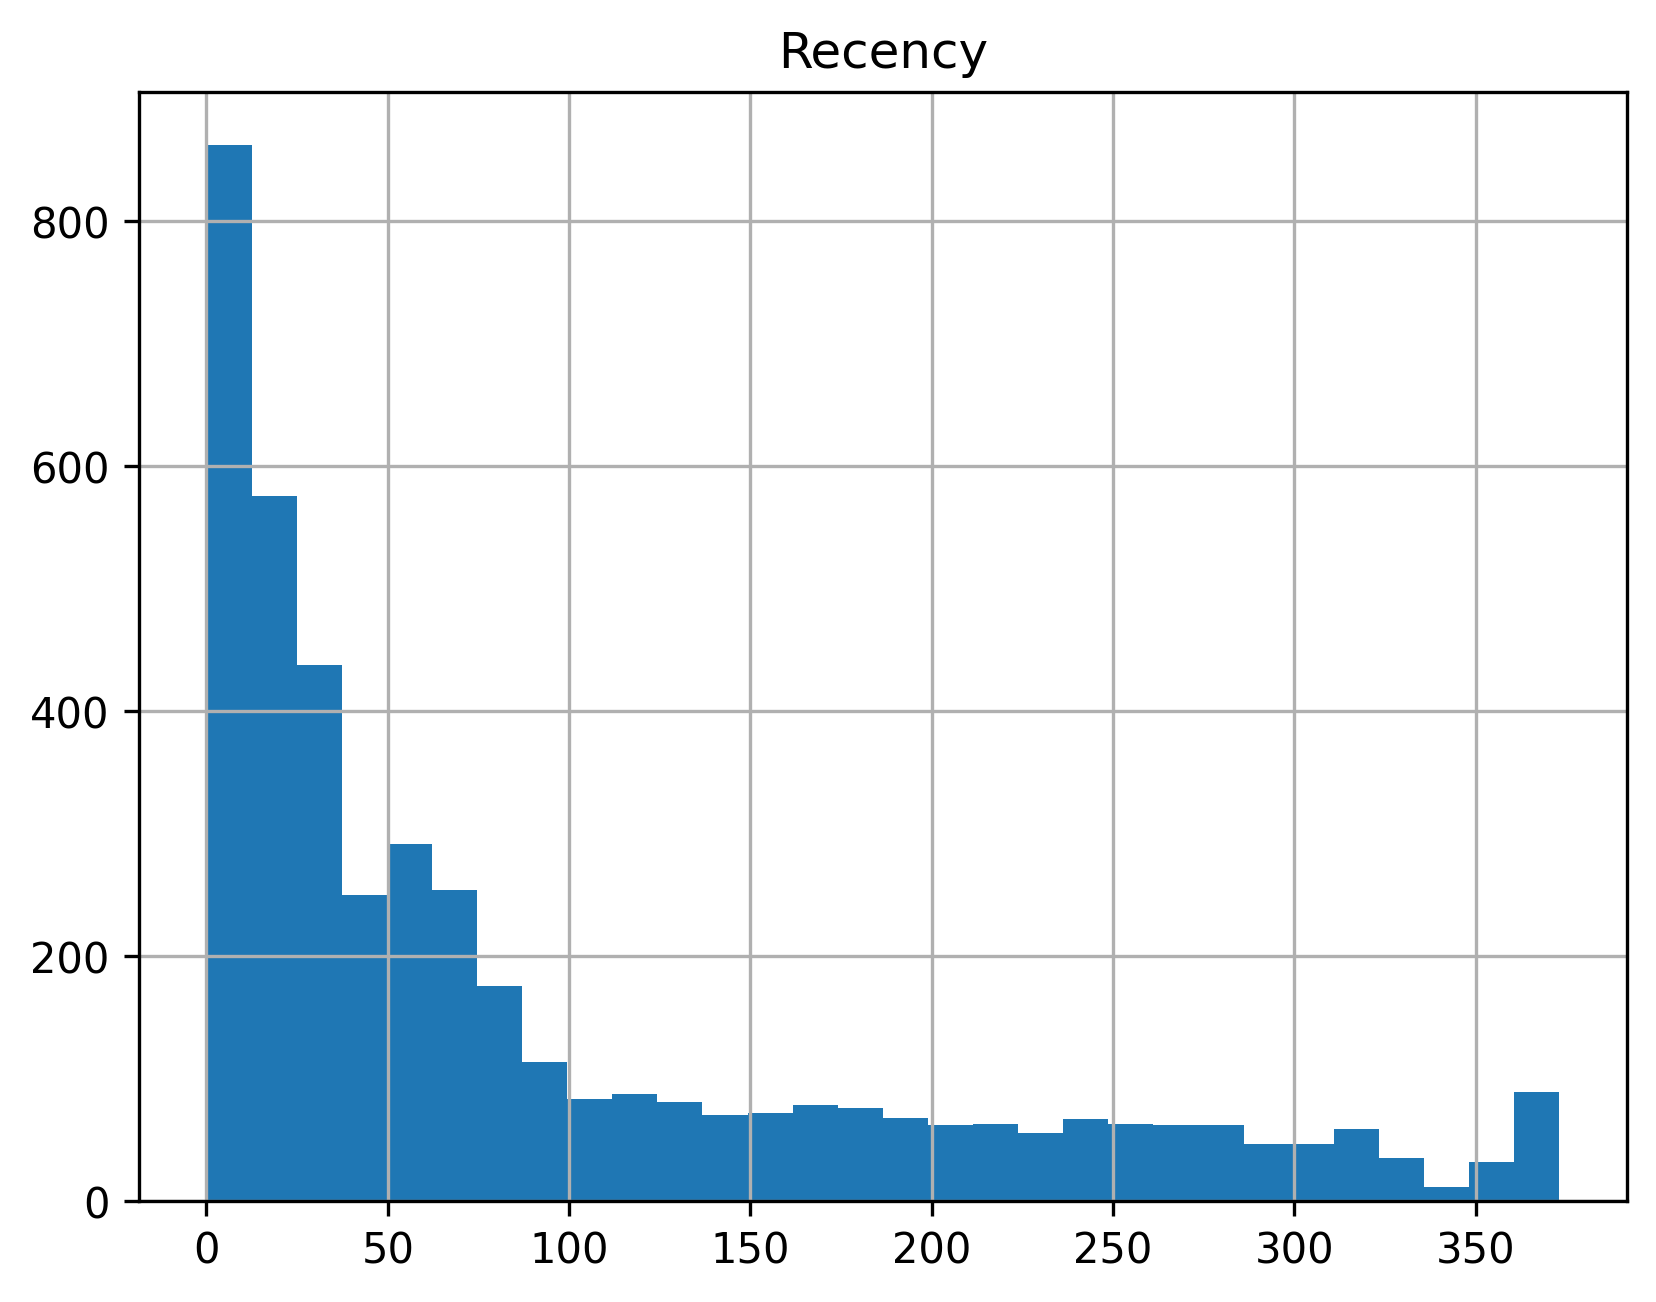
\includegraphics[width=0.9\textwidth]{../report/Figures/recency_distribution_before_scaling.png}
    \caption{Phân phối của Recency trước khi chuẩn hóa}
    \label{fig:recency_distribution}
\end{figure}


\begin{figure}[H]
    \centering
    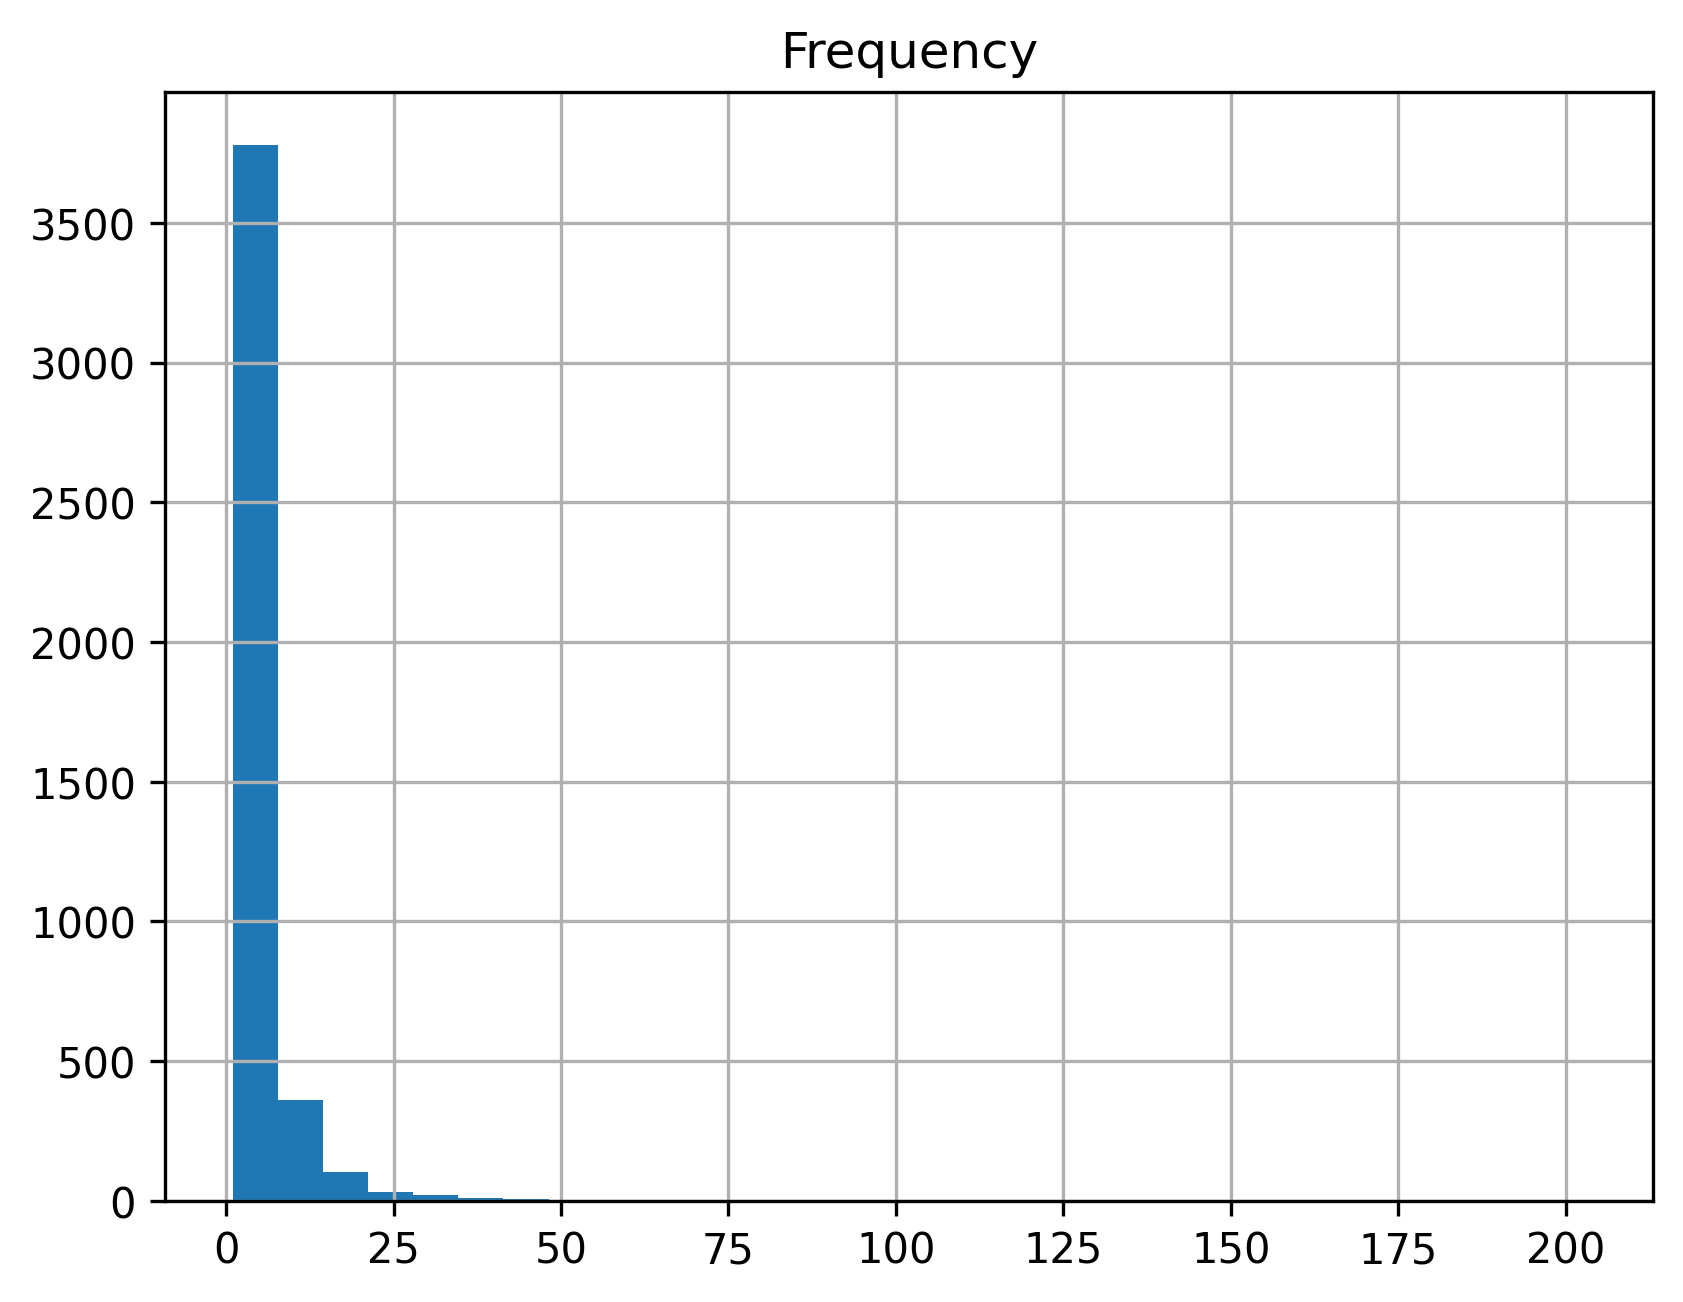
\includegraphics[width=0.9\textwidth]{../report/Figures/frequency_distribution_before_scaling.png}
    \caption{Phân phối của Frequency trước khi chuẩn hóa}
    \label{fig:frequency_distribution}
\end{figure}


\begin{figure}[H]
    \centering
    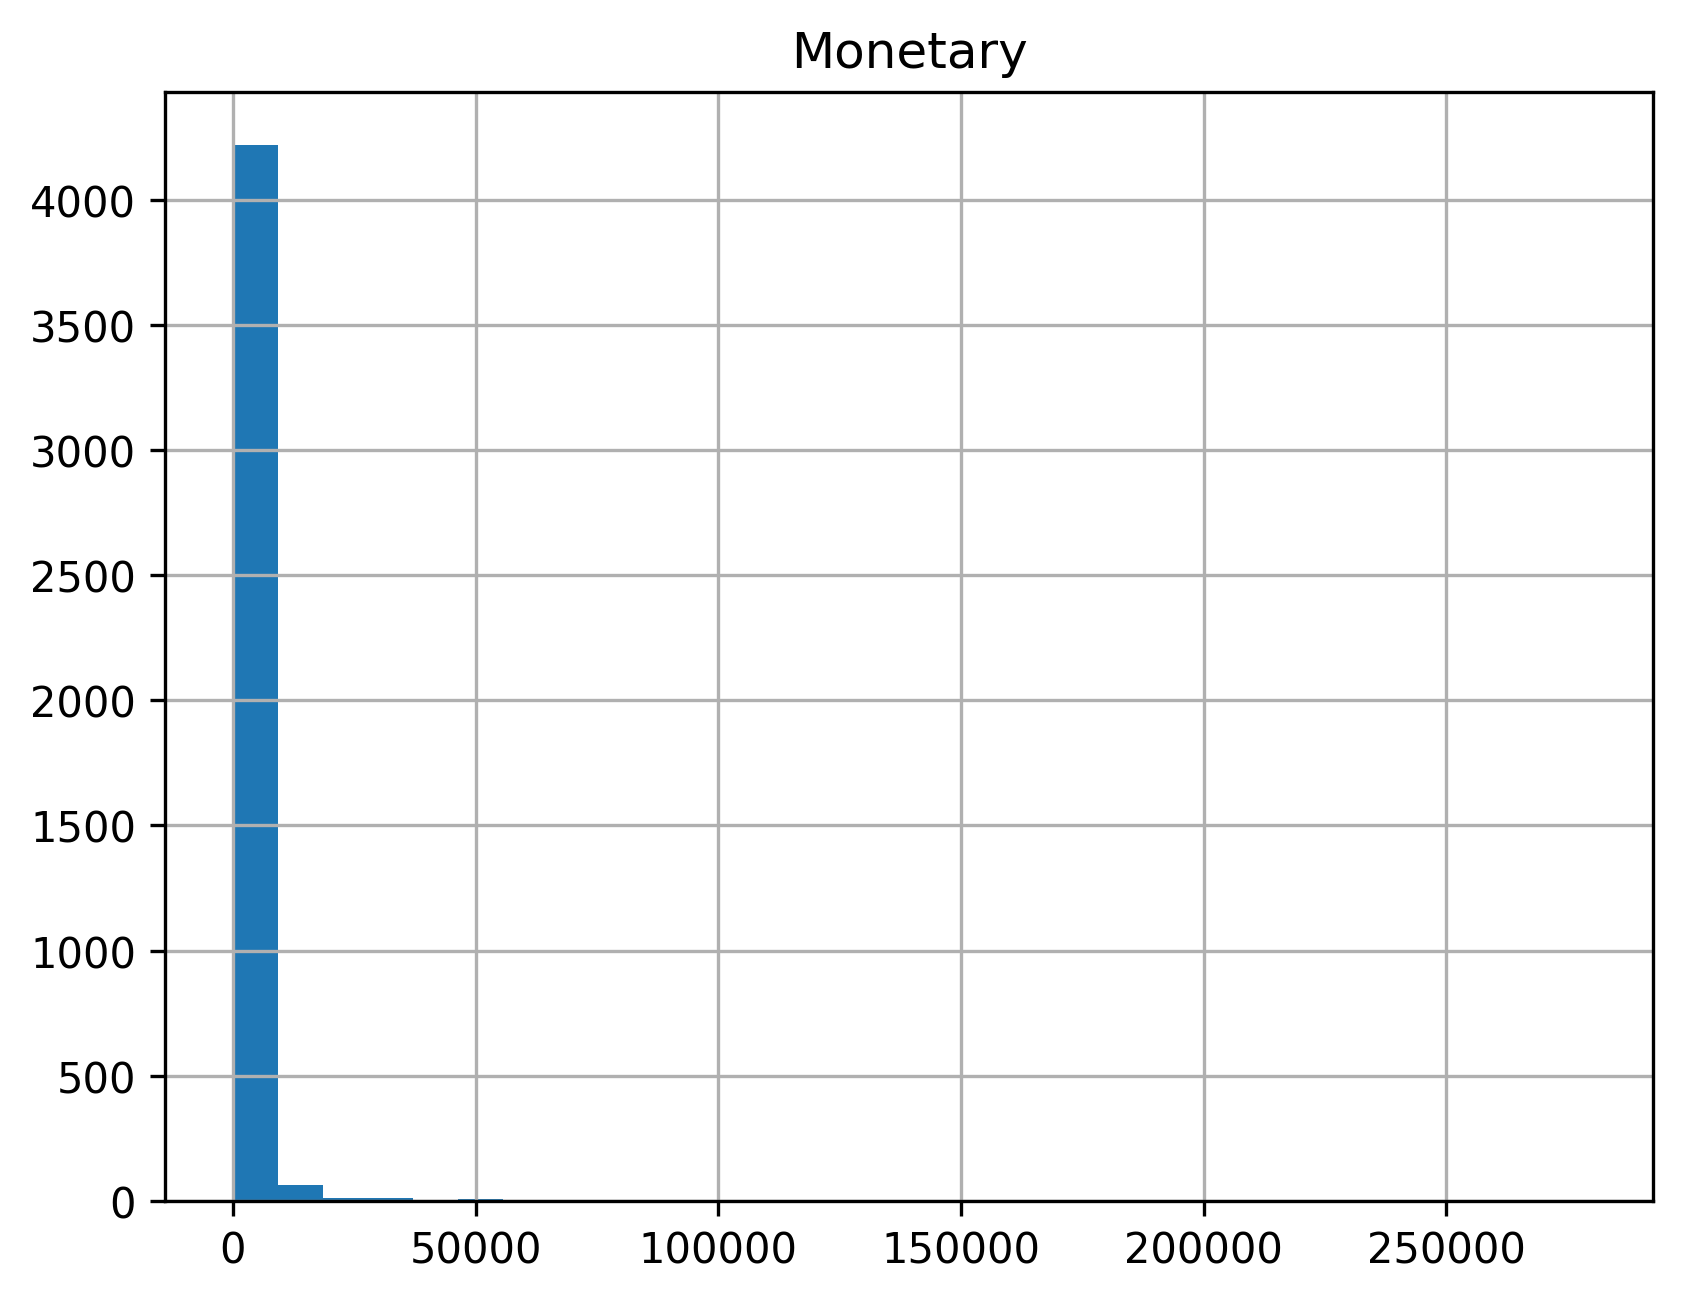
\includegraphics[width=0.9\textwidth]{../report/Figures/monetary_distribution_before_scaling.png}
    \caption{Phân phối của Monetary trước khi chuẩn hóa}
    \label{fig:monetary_distribution}
\end{figure}

Biểu đồ phân phối cho thấy các đặc trưng RFM đều có xu hướng lệch phải, phù hợp với kết quả tính toán hệ số skewness. Trong đó, Monetary thể hiện mức độ lệch mạnh nhất khi phần lớn khách hàng có giá trị chi tiêu thấp, trong khi một số ít khách hàng có tổng chi tiêu rất lớn tạo thành phần đuôi kéo dài của phân phối.

Frequency cũng có hiện tượng tương tự khi đa số khách hàng chỉ thực hiện một số ít giao dịch, nhưng tồn tại một nhóm khách hàng có tần suất mua hàng cao. 

Đối với Recency, phân phối cân đối hơn nhưng vẫn có xu hướng tập trung ở các giá trị nhỏ và kéo dài về phía các khoảng thời gian lớn hơn.

\subsubsection{Biến đổi logarithm và chuẩn hóa đặc trưng}

Kết quả thống kê mô tả cho thấy cả ba đặc trưng RFM đều có phân phối lệch phải, trong đó hai đặc trưng Frequency và Monetary có mức độ lệch lớn nhất. Để giảm ảnh hưởng của các giá trị ngoại lai và đưa hai đặc trưng này về phân phối gần chuẩn hơn, nghiên cứu tiến hành bước \textbf{biến đổi logarithm} cho hai đặc trưng Frequency và Monetary. 

Phép biến đổi được thực hiện theo công thức:

\begin{equation}
x'=\ln(1+x)
\end{equation}

Trong đó, $x$ là giá trị ban đầu và $x'$ là giá trị sau biến đổi. Việc sử dụng hàm $\ln(1+x)$ giúp xử lý trường hợp giá trị bằng 0 và đồng thời làm giảm độ lệch của phân phối.

Kết quả sau bước biến đổi logarithm được trực quan trong Hình \ref{fig:frequency_distribution_after_log_transform} và Hình \ref{fig:monetary_distribution_after_log_transform} dưới đây:

\begin{figure}[H]
    \centering
    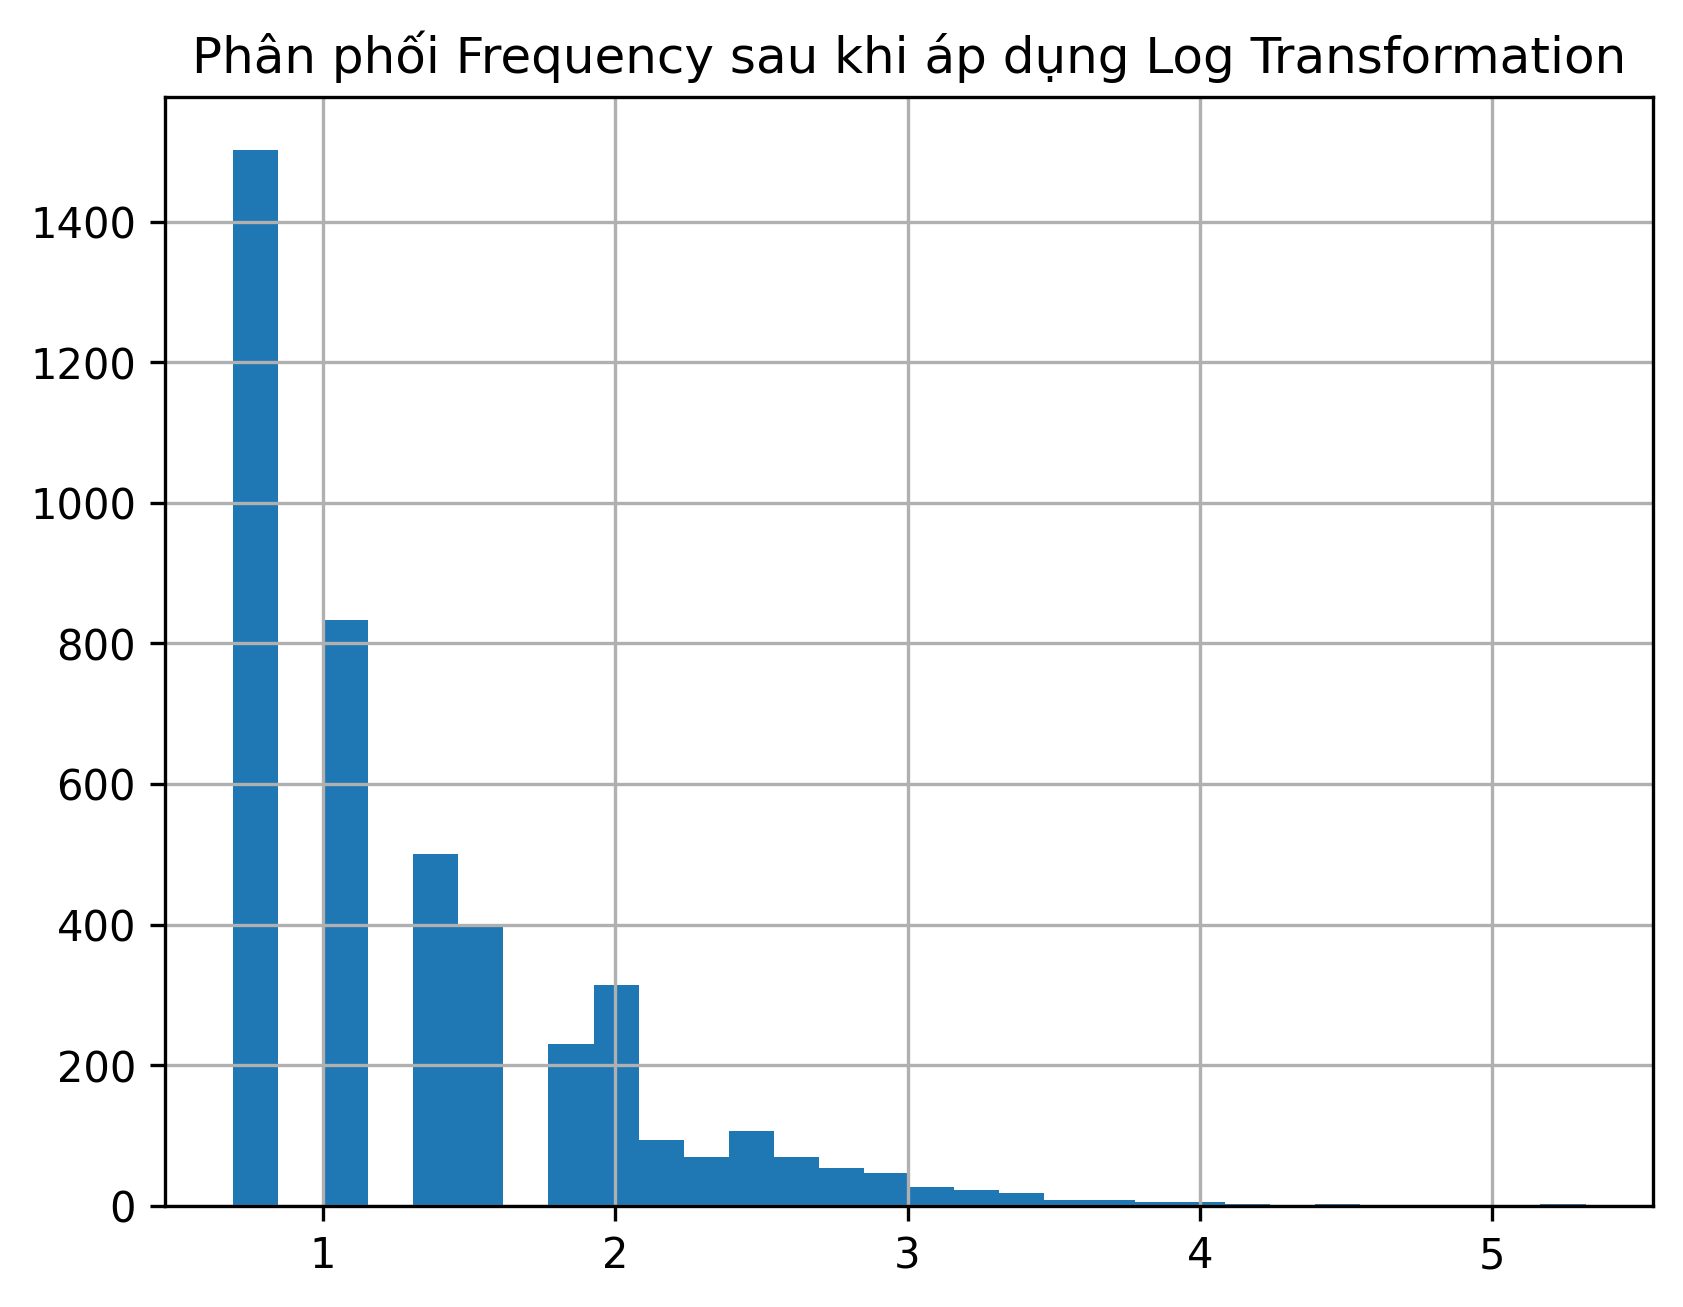
\includegraphics[width=0.9\textwidth]{../report/Figures/frequency_distribution_after_log_transformation.png}
    \caption{Phân phối của Frequency sau bước biến đổi logarithm}
    \label{fig:frequency_distribution_after_log_transform}
\end{figure}

\begin{figure}[H]
    \centering
    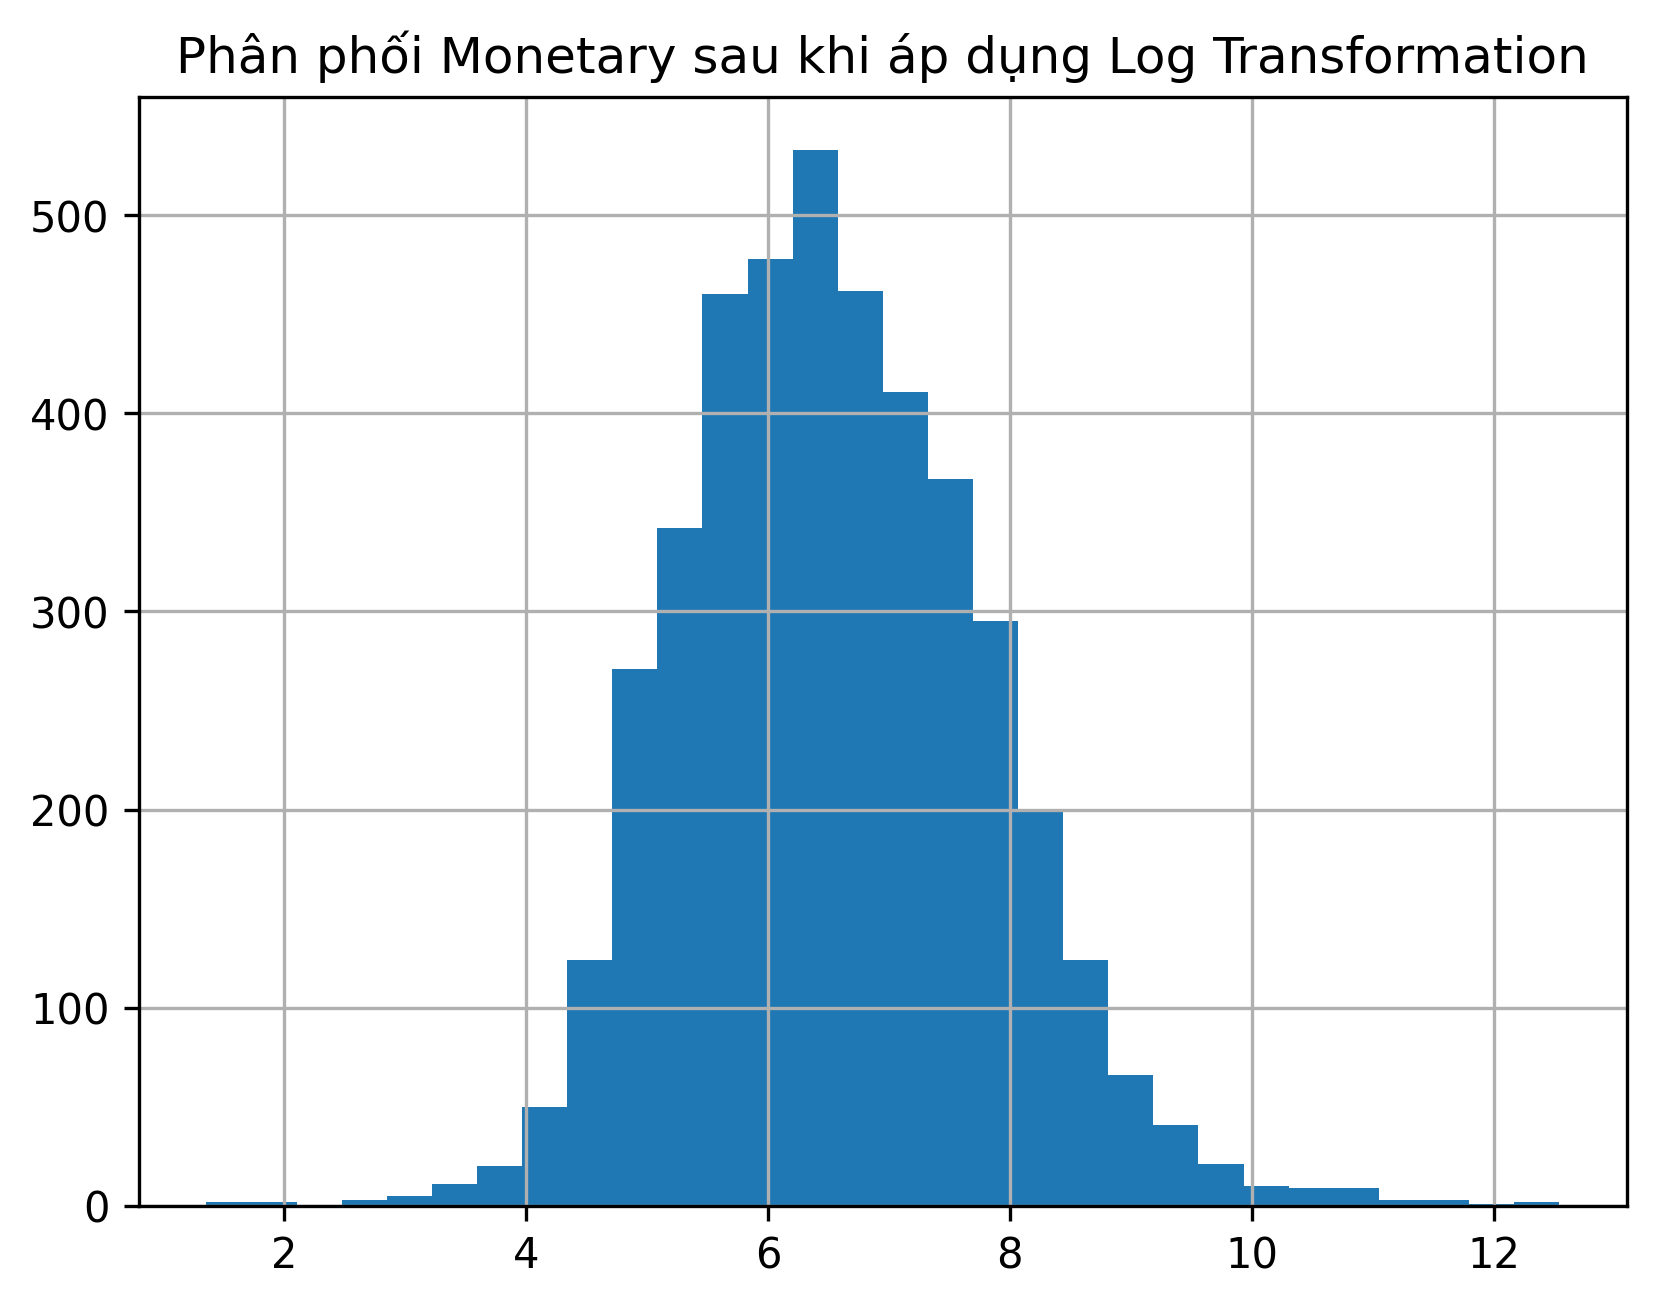
\includegraphics[width=0.9\textwidth]{../report/Figures/monetary_distribution_after_log_transformation.png}
    \caption{Phân phối của Monetary sau bước biến đổi logarithm}
    \label{fig:monetary_distribution_after_log_transform}
\end{figure}

Độ lệch đã giảm đáng kể sang khi áp dụng phương pháp \textdf{biến đổi logarithm}, phân phối Frequency vẫn còn lệch phải nhưng đã giảm từ 11.84 xuống còn 1.92. Trong khi Monetary giảm từ 21.49 xuống còn 1.75, đáng ngạc nhiên là hình dạng phân phối của Monetary xấp xỉ phân phối chuẩn. Điều này cho thấy bước biến đổi logarithm đã giúp cải thiện đáng kể hình dạng phân phối của hai đặc trưng này.

Sau bước \textbf{biến đổi logarithm}, ba đặc trưng gồm Recency, Frequency và Monetary được chuẩn hóa bằng phương pháp \textbf{StandardScaler} nhằm đưa các biến về cùng thang đo. Giá trị chuẩn hóa được tính theo công thức:

\begin{equation}
z=\frac{x-\mu}{\sigma}
\end{equation}

trong đó:

\begin{itemize}
    \item $x$ là giá trị của quan sát;
    \item $\mu$ là giá trị trung bình của đặc trưng;
    \item $\sigma$ là độ lệch chuẩn của đặc trưng.
\end{itemize}

Sau khi chuẩn hóa, mỗi đặc trưng có giá trị trung bình xấp xỉ bằng 0 và độ lệch chuẩn bằng 1. Điều này giúp các biến có cùng mức độ ảnh hưởng trong quá trình tính khoảng cách và hạn chế hiện tượng một đặc trưng có miền giá trị lớn chi phối kết quả phân cụm.

\subsection{Huấn luyện các thuật toán phân cụm}

\subsubsection{Các thuật toán phân cụm}

Dữ liệu sau khi được chuẩn hóa ở bước trên là đầu vào cho các thuật toán phân cụm. Nghiên cứu lựa chọn ba thuật toán phân cụm đại diện cho ba hướng tiếp cận khác nhau trong học máy không giám sát.

\begin{itemize}

\item \textbf{K-Means}: thuật toán phân cụm dựa trên khoảng cách, được sử dụng làm mô hình cơ sở (Baseline).

\item \textbf{Gaussian Mixture Model (GMM)}: thuật toán phân cụm xác suất, cho phép mỗi quan sát có xác suất thuộc nhiều cụm.

\item \textbf{HDBSCAN}: thuật toán phân cụm dựa trên mật độ, có khả năng tự động xác định số cụm và nhận diện các điểm nhiễu.

\end{itemize}

\subsubsection{Không gian tìm kiếm siêu tham số}

Câu hỏi đặt ra là làm thế nào để lựa chọn các siêu tham số tối ưu cho từng thuật toán phân cụm. 

Ý tưởng là thực hiện tìm kiếm trên một không gian siêu tham số đã được xác định trước. Sau khi xác định không gian tìm kiếm, các thuật toán sẽ được huấn luyện trên từng tổ hợp siêu tham số và đánh giá dựa trên các tiêu chí đã đề xuất.

Chính vì vậy, trước tiên, nghiên cứu xác định trước không gian tìm kiếm siêu tham số cho cả ba thuật toán phân cụm. Mỗi mô hình được huấn luyện trên cùng bộ dữ liệu đầu vào và chỉ thay đổi các siêu tham số có ảnh hưởng trực tiếp đến kết quả phân cụm, trong khi các tham số còn lại được giữ cố định. Cách tiếp cận này giúp bảo đảm tính công bằng khi so sánh hiệu quả giữa các thuật toán.

Đối với thuật toán K-Means, các tham số khởi tạo và điều kiện hội tụ được giữ cố định như trình bày trong Bảng~\ref{tab:kmeans_hyperparameter}.

\begin{table}[H]
\centering
\caption{Không gian tìm kiếm siêu tham số của thuật toán K-Means}
\label{tab:kmeans_hyperparameter}
\renewcommand{\arraystretch}{1.3}
\begin{tabular}{ll}
\toprule
\textbf{Siêu tham số} & \textbf{Giá trị} \\
\midrule
\texttt{n\_clusters} & 2, 3, \ldots, 10 \\
\texttt{init} & \texttt{k-means++} \\
\texttt{n\_init} & \texttt{auto} \\
\texttt{max\_iter} & 300 \\
\texttt{random\_state} & 42 \\
\bottomrule
\end{tabular}
\end{table}

Đối với Gaussian Mixture Model (GMM), ngoài việc thay đổi số thành phần Gaussian (\texttt{n\_components}), nghiên cứu còn đánh giá bốn dạng ma trận hiệp phương sai gồm \textit{full}, \textit{tied}, \textit{diag} và \textit{spherical}. Việc khảo sát nhiều dạng ma trận hiệp phương sai giúp đánh giá khả năng mô hình hóa các cụm có hình dạng và mức độ phân tán khác nhau. Các siêu tham số của GMM được trình bày trong Bảng~\ref{tab:gmm_hyperparameter}.

\begin{table}[H]
\centering
\caption{Không gian tìm kiếm siêu tham số của thuật toán Gaussian Mixture Model}
\label{tab:gmm_hyperparameter}
\renewcommand{\arraystretch}{1.3}
\begin{tabular}{ll}
\toprule
\textbf{Siêu tham số} & \textbf{Giá trị} \\
\midrule
\texttt{n\_components} & 2, 3, \ldots, 10 \\
\texttt{covariance\_type} &
\texttt{full}, \texttt{tied}, \texttt{diag}, \texttt{spherical} \\
\texttt{max\_iter} & 300 \\
\texttt{random\_state} & 42 \\
\bottomrule
\end{tabular}
\end{table}


Đối với HDBSCAN, nghiên cứu khảo sát hai siêu tham số quan trọng là \texttt{min\_cluster\_size} và \texttt{min\_samples}. Hai tham số này quyết định kích thước tối thiểu của một cụm và mức độ nghiêm ngặt trong việc xác định mật độ điểm dữ liệu, từ đó ảnh hưởng trực tiếp đến số lượng cụm được phát hiện cũng như khả năng nhận diện các điểm nhiễu. Không gian tìm kiếm của HDBSCAN được trình bày trong Bảng~\ref{tab:hdbscan_hyperparameter}.

\begin{table}[H]
\centering
\caption{Không gian tìm kiếm siêu tham số của thuật toán HDBSCAN}
\label{tab:hdbscan_hyperparameter}
\renewcommand{\arraystretch}{1.3}
\begin{tabular}{ll}
\toprule
\textbf{Siêu tham số} & \textbf{Giá trị} \\
\midrule
\texttt{min\_cluster\_size} & 5, 10, 20, 30, 50 \\
\texttt{min\_samples} & None, 5, 10 \\
\texttt{cluster\_selection\_method} & \texttt{eom} \\
\texttt{metric} & Euclidean \\
\bottomrule
\end{tabular}
\end{table}

Toàn bộ các tổ hợp siêu tham số trong không gian tìm kiếm đều được huấn luyện và đánh giá bằng cùng một quy trình thực nghiệm.

\subsubsection{Đánh giá và so sánh các thuật toán phân cụm}

Sau khi huấn luyện các thuật toán với các cấu hình siêu tham số khác nhau, nghiên cứu tiến hành đánh giá và so sánh kết quả phân cụm dựa trên một khung đánh giá thống nhất. 

Do bài toán phân cụm là bài toán học không giám sát và không có nhãn thực tế (\textit{ground truth}), nghiên cứu không sử dụng các chỉ số đánh giá của bài toán phân loại như Accuracy, Precision hay Recall. Thay vào đó, hiệu quả của các thuật toán được xem xét trên ba tiêu chí gồm: 

\begin{table}[H]
\centering
\caption{Khung tiêu chí đánh giá và so sánh các thuật toán phân cụm}
\label{tab:clustering_evaluation_framework}
\renewcommand{\arraystretch}{1.3}
\begin{tabular}{p{3.5cm}p{3cm}p{5cm}p{3cm}}
\toprule
\textbf{Tiêu chí đánh giá} & 
\textbf{Loại đánh giá} & 
\textbf{Phương pháp đo lường} &
\textbf{Mục đích đánh giá} \\
\midrule

Chất lượng phân cụm &
Định lượng &
Sử dụng các chỉ số đánh giá nội tại gồm Silhouette Score, Davies--Bouldin Index (DBI) và Calinski--Harabasz Index (CHI) &
Đánh giá mức độ liên kết trong cụm và khả năng phân tách giữa các cụm \\

\midrule

Độ ổn định &
Định lượng &
Thực hiện lấy mẫu lại dữ liệu (\textit{resampling}) và đo sự tương đồng giữa các kết quả phân cụm bằng Adjusted Rand Index (ARI) &
Đánh giá khả năng duy trì cấu trúc cụm khi dữ liệu có thay đổi nhỏ \\

\midrule

Khả năng diễn giải và giá trị nghiệp vụ &
Định lượng kết hợp định tính &
Phân tích hồ sơ cụm dựa trên các đặc trưng RFM (giá trị trung bình, trung vị, phân phối), kết hợp trực quan hóa và diễn giải hành vi khách hàng của từng nhóm &
Đánh giá mức độ dễ hiểu của các phân khúc và khả năng ứng dụng kết quả trong hoạt động quản trị khách hàng \\

\bottomrule
\end{tabular}
\end{table}

\paragraph{Đánh giá chất lượng phân cụm:}

Chất lượng phân cụm được đánh giá dựa trên hai khía cạnh chính gồm mức độ tương đồng giữa các điểm dữ liệu trong cùng một cụm và mức độ phân biệt giữa các cụm khác nhau. Nghiên cứu sử dụng ba chỉ số đánh giá nội tại gồm Silhouette Score, Davies--Bouldin Index (DBI) và Calinski--Harabasz Index (CHI).

\begin{itemize}

\item \textbf{Silhouette Score:}

Silhouette Score đo lường mức độ phù hợp của một điểm dữ liệu với cụm mà nó được gán bằng cách so sánh khoảng cách trung bình trong cùng cụm và khoảng cách đến cụm gần nhất khác. Với một điểm dữ liệu $i$, hệ số Silhouette được xác định như sau:

\begin{equation}
s(i)=\frac{b(i)-a(i)}
{\max(a(i),b(i))}
\end{equation}

Trong đó:

\begin{itemize}
    \item $a(i)$ là khoảng cách trung bình từ điểm $i$ đến các điểm khác trong cùng một cụm.
    \item $b(i)$ là khoảng cách trung bình nhỏ nhất từ điểm $i$ đến các điểm thuộc cụm khác gần nhất.
\end{itemize}

Giá trị Silhouette Score của toàn bộ mô hình được tính bằng trung bình của $s(i)$ trên toàn bộ điểm dữ liệu:

\begin{equation}
S=\frac{1}{n}\sum_{i=1}^{n}s(i)
\end{equation}

Giá trị $S$ nằm trong khoảng $[-1,1]$. Giá trị càng lớn cho thấy các cụm có mức độ kết dính cao và khả năng phân tách tốt.


\item \textbf{Davies--Bouldin Index (DBI):}

Davies--Bouldin Index đánh giá mức độ tương đồng giữa các cụm dựa trên tỷ lệ giữa độ phân tán trong cụm và khoảng cách giữa các tâm cụm. Chỉ số được xác định như sau:

\begin{equation}
DBI=\frac{1}{k}
\sum_{i=1}^{k}
\max_{j\neq i}
\left(
\frac{S_i+S_j}{M_{ij}}
\right)
\end{equation}

Trong đó:

\begin{itemize}
    \item $k$ là số lượng cụm.
    \item $S_i$ và $S_j$ là độ phân tán của cụm $i$ và cụm $j$.
    \item $M_{ij}$ là khoảng cách giữa tâm của hai cụm $i$ và $j$.
\end{itemize}

Giá trị DBI càng nhỏ thể hiện các cụm càng khác biệt và mô hình có chất lượng phân cụm tốt hơn.


\item \textbf{Calinski--Harabasz Index (CHI):}

Calinski--Harabasz Index đo lường tỷ lệ giữa mức độ phân tán giữa các cụm và mức độ phân tán bên trong cụm:

\begin{equation}
CH=
\frac{Tr(B_k)}
{Tr(W_k)}
\times
\frac{n-k}{k-1}
\end{equation}

Trong đó:

\begin{itemize}
    \item $n$ là số lượng quan sát.
    \item $k$ là số lượng cụm.
    \item $B_k$ biểu diễn ma trận phân tán giữa các cụm.
    \item $W_k$ biểu diễn ma trận phân tán trong cụm.
\end{itemize}

Giá trị CHI càng lớn cho thấy sự khác biệt giữa các cụm càng rõ ràng.

\end{itemize}


\paragraph{Đánh giá độ ổn định của kết quả phân cụm:}

Độ ổn định phản ánh khả năng duy trì cấu trúc phân cụm của thuật toán khi dữ liệu đầu vào có những thay đổi nhỏ. Nghiên cứu đánh giá tiêu chí này bằng phương pháp lấy mẫu lại (\textit{resampling}) kết hợp với chỉ số Adjusted Rand Index (ARI).

Từ tập dữ liệu ban đầu $D$, tạo ra $m$ tập dữ liệu con thông qua quá trình lấy mẫu:

\begin{equation}
D_1,D_2,...,D_m
\end{equation}

Mỗi tập dữ liệu được sử dụng để huấn luyện lại thuật toán với cùng cấu hình siêu tham số. Kết quả phân cụm giữa các lần chạy được ký hiệu là:

\begin{equation}
C_1,C_2,...,C_m
\end{equation}

Độ tương đồng giữa hai kết quả phân cụm được đo bằng Adjusted Rand Index:

\begin{equation}
ARI=
\frac{RI-E(RI)}
{\max(RI)-E(RI)}
\end{equation}

Trong đó:

\begin{itemize}
    \item $RI$ là Rand Index, đo mức độ đồng thuận giữa hai cách phân nhóm.
    \item $E(RI)$ là giá trị kỳ vọng của Rand Index khi phân nhóm xảy ra ngẫu nhiên.
\end{itemize}

Giá trị ARI nằm trong khoảng $[-1,1]$, trong đó giá trị càng gần 1 thể hiện các kết quả phân cụm càng ổn định qua các lần lấy mẫu khác nhau.

\paragraph{Đánh giá khả năng diễn giải và ý nghĩa nghiệp vụ:}

Bên cạnh các chỉ số định lượng, nghiên cứu đánh giá khả năng diễn giải của kết quả phân cụm thông qua việc xây dựng hồ sơ khách hàng (\textit{cluster profile}) cho từng nhóm được tạo ra.

Đối với mỗi cụm khách hàng, các thống kê mô tả của ba đặc trưng RFM gồm: \textbf{giá trị trung bình}, \textbf{trung vị} và \textbf{phân phối} của Recency, Frequency và Monetary được phân tích nhằm xác định sự khác biệt về hành vi mua sắm giữa các nhóm.

Một kết quả phân cụm được xem là có khả năng diễn giải tốt khi các cụm thể hiện được những đặc điểm hành vi riêng biệt, chẳng hạn như nhóm khách hàng có giá trị cao, nhóm khách hàng mua thường xuyên hoặc nhóm khách hàng có dấu hiệu giảm tương tác. Các đặc điểm này giúp đánh giá mức độ hữu ích của kết quả phân cụm trong các hoạt động quản trị quan hệ khách hàng.

\paragraph{So sánh tổng hợp giữa các thuật toán:}

Sau khi đánh giá từng thuật toán trên ba nhóm tiêu chí gồm chất lượng phân cụm, độ ổn định và khả năng diễn giải cùng giá trị nghiệp vụ, nghiên cứu thực hiện so sánh tổng hợp nhằm xác định sự khác biệt giữa K-Means, Gaussian Mixture Model (GMM) và HDBSCAN.

Do mỗi tiêu chí phản ánh một khía cạnh khác nhau của hiệu quả phân cụm, nghiên cứu không sử dụng một chỉ số duy nhất để quyết định thuật toán tốt nhất. Thay vào đó, kết quả được tổng hợp theo hướng đánh giá đa tiêu chí (\textit{multi-criteria evaluation}), trong đó từng thuật toán được xem xét dựa trên mức độ đáp ứng của từng tiêu chí riêng biệt.

Đối với tiêu chí chất lượng phân cụm, các thuật toán được so sánh dựa trên sự kết hợp của ba chỉ số nội tại gồm Silhouette Score, Davies--Bouldin Index và Calinski--Harabasz Index. Thuật toán được đánh giá cao hơn khi tạo ra các cụm có mức độ kết dính lớn, khả năng phân tách tốt và cấu trúc cụm rõ ràng.

Đối với tiêu chí độ ổn định, kết quả phân cụm qua nhiều lần lấy mẫu lại được so sánh thông qua giá trị Adjusted Rand Index (ARI). Thuật toán có giá trị ARI cao hơn được xem là có khả năng duy trì cấu trúc phân cụm tốt hơn trước sự thay đổi nhỏ của dữ liệu.

Đối với tiêu chí khả năng diễn giải và giá trị nghiệp vụ, nghiên cứu phân tích hồ sơ của từng cụm dựa trên các đặc trưng RFM. Các thuật toán được đánh giá dựa trên khả năng tạo ra các nhóm khách hàng có đặc điểm hành vi rõ ràng, có thể mô tả bằng các nhóm khách hàng cụ thể và hỗ trợ cho việc ra quyết định trong quản trị quan hệ khách hàng.

Cuối cùng, kết quả của ba nhóm tiêu chí được tổng hợp để phân tích ưu điểm, hạn chế và điều kiện phù hợp của từng thuật toán. Một thuật toán chỉ được xem là phù hợp hơn khi đạt được sự cân bằng giữa khả năng tạo cụm tốt, tính ổn định của kết quả và mức độ hữu ích trong việc diễn giải hành vi khách hàng.

Cách tiếp cận này giúp nghiên cứu tránh việc kết luận dựa trên một tiêu chí đơn lẻ và cung cấp đánh giá toàn diện hơn về sự phù hợp của từng thuật toán trong bài toán Customer Segmentation trên bộ dữ liệu Online Retail II.

\subsubsection{Phân tích và diễn giải ý nghĩa nghiệp vụ}

Sau khi lựa chọn được thuật toán phân cụm phù hợp nhất, nghiên cứu tiến hành phân tích đặc điểm của từng cụm khách hàng nhằm đánh giá khả năng ứng dụng của kết quả phân cụm trong bối cảnh quản trị quan hệ khách hàng (CRM). Mục tiêu của bước này không phải là đánh giá lại chất lượng thuật toán mà là diễn giải các nhóm khách hàng dưới góc nhìn nghiệp vụ.

Đối với mỗi cụm, nghiên cứu tính toán các thống kê mô tả của ba đặc trưng Recency, Frequency và Monetary, bao gồm giá trị trung bình, trung vị và độ phân tán. Các thống kê này được sử dụng để xây dựng hồ sơ (Cluster Profile) cho từng nhóm khách hàng và so sánh sự khác biệt về hành vi mua sắm giữa các cụm.

\subsection{Cấu hình thực nghiệm}

Để đảm bảo khả năng tái lập của nghiên cứu, toàn bộ quá trình thực nghiệm được thực hiện trong một môi trường tính toán thống nhất. Các thuật toán phân cụm, quá trình tối ưu siêu tham số và các bước đánh giá mô hình đều được triển khai trên cùng một cấu hình phần mềm.

\subsubsection{Môi trường phần mềm}

Nghiên cứu sử dụng ngôn ngữ lập trình Python để triển khai toàn bộ quy trình xử lý dữ liệu, xây dựng đặc trưng RFM, huấn luyện mô hình phân cụm và đánh giá kết quả. Các thư viện chính được sử dụng bao gồm:

\begin{itemize}
    \item \texttt{pandas}: xử lý và biến đổi dữ liệu giao dịch.
    \item \texttt{numpy}: thực hiện các phép toán số học.
    \item \texttt{scikit-learn}: triển khai K-Means, Gaussian Mixture Model, chuẩn hóa dữ liệu và các chỉ số đánh giá phân cụm.
    \item \texttt{hdbscan}: triển khai thuật toán HDBSCAN.
    \item \texttt{matplotlib} và \texttt{seaborn}: trực quan hóa kết quả phân tích.
\end{itemize}

\subsubsection{Thiết lập thực nghiệm chung}

Để đảm bảo tính công bằng khi so sánh giữa các thuật toán, toàn bộ mô hình được huấn luyện trên cùng một tập dữ liệu đầu vào sau khi đã hoàn thành các bước tiền xử lý, xây dựng đặc trưng RFM và chuẩn hóa dữ liệu.

Các thiết lập chung trong quá trình thực nghiệm bao gồm:

\begin{itemize}
    \item Sử dụng cùng bộ đặc trưng RFM làm đầu vào cho cả ba thuật toán K-Means, Gaussian Mixture Model (GMM) và HDBSCAN.
    \item Áp dụng cùng quy trình chuẩn hóa dữ liệu trước khi phân cụm.
    \item Sử dụng cùng phương pháp đánh giá dựa trên chất lượng phân cụm, độ ổn định và khả năng diễn giải.
    \item Cố định giá trị \texttt{random\_state}=42 đối với các thuật toán có yếu tố ngẫu nhiên nhằm đảm bảo khả năng tái lập kết quả.
\end{itemize}

Các thiết lập trên giúp loại bỏ ảnh hưởng từ sự khác biệt trong quá trình xử lý dữ liệu và tập trung đánh giá sự khác biệt đến từ bản chất của từng thuật toán phân cụm.

Toàn bộ các thuật toán được huấn luyện trên cùng bộ dữ liệu RFM đã chuẩn hóa và đánh giá theo cùng một quy trình thực nghiệm. Việc cố định dữ liệu đầu vào, quy trình tiền xử lý và các tham số chung giúp đảm bảo tính công bằng khi so sánh hiệu quả của các thuật toán phân cụm, đồng thời tăng khả năng tái lập của nghiên cứu.

% --------------------------------------------------------------------------
\section{Kết quả và thảo luận}

\subsection{Đánh giá chất lượng phân cụm}

\subsubsection{Kết quả thực nghiệm}

Để trả lời tiêu chí đầu tiên của câu hỏi nghiên cứu, các thuật toán K-Means, Gaussian Mixture Model (GMM) và HDBSCAN được huấn luyện trên cùng bộ dữ liệu RFM đã chuẩn hóa. Với mỗi thuật toán, nghiên cứu lựa chọn cấu hình siêu tham số cho kết quả tốt nhất theo hệ thống chỉ số đánh giá nội tại gồm Silhouette Score, Davies--Bouldin Index (DBI) và Calinski--Harabasz Index (CHI). Đối với HDBSCAN, số lượng điểm nhiễu (\textit{Noise}) cũng được ghi nhận do đây là một phần trong cơ chế hoạt động của thuật toán.

Kết quả đánh giá của ba thuật toán được trình bày trong Bảng~\ref{tab:clustering_quality_result}.

\begin{table}[H]
\centering
\caption{Kết quả đánh giá chất lượng phân cụm của các thuật toán}
\label{tab:clustering_quality_result}
\renewcommand{\arraystretch}{1.2}
\begin{tabular}{lcccccc}
\toprule
\textbf{Thuật toán} &
\textbf{Số cụm} &
\textbf{Noise} &
\textbf{Silhouette} &
\textbf{DBI} &
\textbf{CHI} \\
\midrule
K-Means & 3 & 0 & 0.414329 & 0.829263 & 4389.590 \\
GMM & 3 & 0 & \textbf{0.414446} & \textbf{0.816665} & 4364.692 \\
HDBSCAN & 3 & 854 & 0.202819 & 1.195553 & 2404.568 \\
\bottomrule
\end{tabular}
\end{table}

\subsubsection{Phân tích và thảo luận}

Kết quả trong Bảng~\ref{tab:clustering_quality_result} cho thấy K-Means và GMM đạt chất lượng phân cụm gần như tương đương. Nhận định này được thể hiện qua việc cả hai thuật toán đều có Silhouette Score xấp xỉ 0.414, Davies--Bouldin Index nhỏ hơn 0.83 và Calinski--Harabasz Index lớn hơn 4360. Sự chênh lệch giữa các chỉ số là rất nhỏ, cho thấy hai thuật toán hình thành cấu trúc cụm có mức độ gắn kết và phân tách tương đương trên không gian đặc trưng RFM.

Trong khi đó, HDBSCAN cho chất lượng phân cụm thấp hơn so với hai thuật toán còn lại. Bằng chứng là Silhouette Score chỉ đạt 0.202819, thấp hơn khoảng một nửa so với K-Means và GMM; đồng thời Davies--Bouldin Index lớn nhất và Calinski--Harabasz Index nhỏ nhất trong ba mô hình. Kết quả này cho thấy các cụm được tạo bởi HDBSCAN có mức độ phân tách kém hơn và độ gắn kết trong cụm thấp hơn trên bộ dữ liệu nghiên cứu.

Một điểm đáng chú ý là HDBSCAN xác định 854 khách hàng là điểm nhiễu, trong khi K-Means và GMM đều phân cụm toàn bộ 4\,324 khách hàng. Việc loại bỏ một tỷ lệ đáng kể quan sát có thể ảnh hưởng đến các chỉ số đánh giá nội tại, bởi các chỉ số này chỉ được tính trên các khách hàng được gán vào cụm.

Từ các kết quả trên có thể thấy K-Means và GMM đạt chất lượng phân cụm cao hơn HDBSCAN theo các chỉ số nội tại. Tuy nhiên, chất lượng phân cụm chỉ phản ánh mức độ phân tách của các cụm tại một thời điểm và chưa cho biết kết quả có được duy trì khi dữ liệu thay đổi hay không. Vì vậy, nghiên cứu tiếp tục đánh giá độ ổn định của các thuật toán trong mục tiếp theo.

\subsection{Đánh giá độ ổn định của kết quả phân cụm}

\subsubsection{Kết quả thực nghiệm}

Bên cạnh chất lượng phân cụm, nghiên cứu tiếp tục đánh giá độ ổn định của các thuật toán khi dữ liệu đầu vào có sự thay đổi. Theo quy trình thực nghiệm đã trình bày ở Chương~3, mỗi thuật toán được huấn luyện lặp lại 50 lần trên các tập dữ liệu được tạo bằng phương pháp lấy mẫu lại (\textit{resampling}). Độ ổn định được đánh giá thông qua ba góc nhìn khác nhau.

Thứ nhất, nghiên cứu tính Adjusted Rand Index (ARI) giữa mọi cặp kết quả phân cụm trong 50 lần lặp. Với 50 lần thực nghiệm, mỗi thuật toán tạo ra $\binom{50}{2}=1225$ cặp so sánh. Đối với mỗi cặp, ARI chỉ được tính trên các khách hàng đồng thời xuất hiện trong cả hai tập mẫu nhằm bảo đảm hai kết quả phân cụm được so sánh trên cùng tập quan sát.

Kết quả thống kê của Pairwise ARI được trình bày trong Bảng~\ref{tab:pairwise_ari}.

\begin{table}[H]
\centering
\caption{Thống kê Pairwise ARI giữa các lần lấy mẫu}
\label{tab:pairwise_ari}
\renewcommand{\arraystretch}{1.2}
\begin{tabular}{lcccc}
\toprule
\textbf{Thuật toán} &
\textbf{Mean} &
\textbf{Std} &
\textbf{Min} &
\textbf{Max} \\
\midrule
K-Means & 0.9751 & 0.0136 & 0.9293 & 0.9989\\
GMM & 0.9747 & 0.0143 & 0.9206 & 1.0000\\
HDBSCAN & 0.9543 & 0.0506 & 0.6894 & 0.9811\\
\bottomrule
\end{tabular}
\end{table}

Để kiểm chứng thêm kết quả trên, nghiên cứu tiếp tục đánh giá khả năng tái tạo cấu trúc phân cụm ban đầu. Cụ thể, kết quả của từng lần lấy mẫu được so sánh với kết quả huấn luyện trên toàn bộ tập dữ liệu gồm 4\,324 khách hàng bằng chỉ số Reference ARI. Chỉ số này phản ánh mức độ mà mô hình duy trì được cấu trúc phân cụm khi dữ liệu đầu vào thay đổi.

Kết quả được trình bày trong Bảng~\ref{tab:reference_ari}.

\begin{table}[H]
\centering
\caption{Reference ARI so với mô hình huấn luyện trên toàn bộ dữ liệu}
\label{tab:reference_ari}
\renewcommand{\arraystretch}{1.2}
\begin{tabular}{lccc}
\toprule
\textbf{Thuật toán} &
\textbf{Mean} &
\textbf{Std} &
\textbf{Min} \\
\midrule
K-Means & 0.9811 & 0.0094 & 0.9599\\
GMM & 0.9814 & 0.0096 & 0.9581\\
HDBSCAN & 0.8918 & 0.0365 & 0.6424\\
\bottomrule
\end{tabular}
\end{table}

Do HDBSCAN có cơ chế nhận diện các điểm nhiễu, sự thay đổi của tập điểm nhiễu giữa các lần lấy mẫu có thể làm giảm chỉ số ARI mặc dù cấu trúc các cụm chính vẫn được giữ nguyên. Vì vậy, nghiên cứu tiếp tục tính lại Pairwise ARI của HDBSCAN sau khi loại bỏ toàn bộ các điểm nhiễu trước khi so sánh.

Kết quả được trình bày trong Bảng~\ref{tab:hdbscan_noise}.

\begin{table}[H]
\centering
\caption{Pairwise ARI của HDBSCAN trước và sau khi loại bỏ điểm nhiễu}
\label{tab:hdbscan_noise}
\renewcommand{\arraystretch}{1.2}
\begin{tabular}{lcc}
\toprule
\textbf{Điều kiện đánh giá} &
\textbf{Mean ARI} &
\textbf{Std} \\
\midrule
Bao gồm điểm nhiễu & 0.9543 & 0.0506\\
Loại bỏ điểm nhiễu & 0.9953 & 0.0231\\
\bottomrule
\end{tabular}
\end{table}

\subsubsection{Phân tích và thảo luận}

\subsection{Phân tích và thảo luận}

Kết quả Pairwise ARI trong Bảng~\ref{tab:pairwise_ari} cho thấy K-Means và GMM có độ ổn định gần như tương đương. Điều này được thể hiện qua giá trị ARI trung bình đều xấp xỉ 0.975 và độ lệch chuẩn nhỏ hơn 0.015, chứng tỏ cấu trúc phân cụm hầu như không thay đổi giữa các lần lấy mẫu. Ngược lại, HDBSCAN có ARI trung bình thấp hơn (0.9543) và độ lệch chuẩn lớn hơn đáng kể (0.0506), phản ánh kết quả phân cụm nhạy cảm hơn trước sự thay đổi của dữ liệu.

Nhận định trên tiếp tục được củng cố bởi kết quả Reference ARI trong Bảng~\ref{tab:reference_ari}. Cả K-Means và GMM đều đạt giá trị trung bình khoảng 0.981, cho thấy các mô hình có khả năng tái tạo gần như toàn bộ cấu trúc phân cụm khi huấn luyện trên các tập dữ liệu con. Trong khi đó, HDBSCAN chỉ đạt 0.8918, cho thấy mức độ tái tạo thấp hơn rõ rệt.

Tuy nhiên, kết quả trong Bảng~\ref{tab:hdbscan_noise} cho thấy nguyên nhân của sự suy giảm này chủ yếu đến từ cơ chế phát hiện điểm nhiễu. Sau khi loại bỏ các điểm nhiễu khỏi phép so sánh, Pairwise ARI của HDBSCAN tăng từ 0.9543 lên 0.9953. Điều này cho thấy cấu trúc của các cụm chính vẫn được duy trì ổn định giữa các lần thực nghiệm; sự khác biệt chủ yếu nằm ở việc một số khách hàng được phân loại là điểm nhiễu hoặc được gán vào cụm tùy theo từng lần lấy mẫu.

Như vậy, xét về độ ổn định, K-Means và GMM duy trì kết quả phân cụm nhất quán hơn trên toàn bộ dữ liệu. Đối với HDBSCAN, sự biến động chủ yếu xuất phát từ quá trình xác định điểm nhiễu thay vì sự thay đổi của cấu trúc cụm. Do đó, để đánh giá đầy đủ hiệu quả của các thuật toán, cần tiếp tục xem xét liệu các cụm tạo ra có dễ diễn giải và mang ý nghĩa nghiệp vụ đối với bài toán phân khúc khách hàng hay không.

\subsection{Khả năng diễn giải và ý nghĩa nghiệp vụ của các cụm}

\subsubsection{Kết quả}

Sau khi đánh giá chất lượng phân cụm và độ ổn định, nghiên cứu tiếp tục xem xét liệu các cụm được tạo thành có thể diễn giải thành những phân khúc khách hàng có ý nghĩa hay không. Để đánh giá tiêu chí này, nghiên cứu lần lượt phân tích (i) mức độ phân biệt giữa các cụm trên ba đặc trưng RFM và (ii) hồ sơ hành vi của từng cụm sau khi gán nhãn nghiệp vụ.

Trước hết, mức độ phân biệt giữa các cụm được đo bằng khoảng cách giữa giá trị trung bình lớn nhất và nhỏ nhất trên từng đặc trưng RFM sau chuẩn hóa. Kết quả được trình bày trong Bảng~\ref{tab:cluster_separation}.

\begin{table}[H]
\centering
\caption{Mức độ phân biệt giữa các cụm trên ba đặc trưng RFM}
\label{tab:cluster_separation}

\renewcommand{\arraystretch}{1.25}

\begin{tabular}{lccccc}
\toprule
\textbf{Thuật toán} &
$\Delta_{R}$ &
$\Delta_{F}$ &
$\Delta_{M}$ &
$\Delta_{mean}$ &
$\Delta_{min}$\\
\midrule
K-Means & 2.246 & 1.953 & 1.888 & 2.029 & 1.888\\
GMM & 2.291 & 1.983 & 1.939 & \textbf{2.071} & \textbf{1.939}\\
HDBSCAN & 1.253 & 1.708 & 1.487 & 1.483 & 1.253\\
\bottomrule
\end{tabular}

\vspace{0.3cm}

\footnotesize
$\Delta_j$ là khoảng cách giữa giá trị trung bình lớn nhất và nhỏ nhất của đặc trưng $j$
sau chuẩn hóa. Vì dữ liệu đã được StandardScaler chuẩn hóa nên $\sigma_j=1$,
do đó $\Delta_j$ được biểu diễn theo số độ lệch chuẩn.
\end{table}

Kết quả cho thấy GMM đạt mức phân biệt trung bình lớn nhất ($\Delta_{mean}=2.071$), tiếp theo là K-Means ($2.029$), trong khi HDBSCAN chỉ đạt $1.483$. Giá trị $\Delta_{min}$ của GMM ($1.939$) và K-Means ($1.888$) cũng lớn hơn đáng kể so với HDBSCAN ($1.253$), cho thấy các cụm của hai thuật toán này được tách biệt rõ hơn trên cả ba đặc trưng RFM.

Để quan sát trực quan sự khác biệt giữa các cụm, Hình~\ref{fig:cluster_profile_bar} trình bày giá trị trung bình chuẩn hóa của từng cụm trên ba đặc trưng Recency, Frequency và Monetary, trong khi Hình~\ref{fig:cluster_profile_radar} biểu diễn cùng thông tin dưới dạng biểu đồ radar.
\begin{figure}[H]
\centering
\includegraphics[width=\textwidth]{figures/chapter4/rfm_bar.png}
\caption{Giá trị trung bình chuẩn hóa của các cụm trên ba đặc trưng RFM}
\label{fig:cluster_profile_bar}
\end{figure}

% Hình Radar

Quan sát hai hình cho thấy K-Means và GMM đều hình thành ba cụm với đặc trưng hành vi khác biệt rõ ràng: một cụm có Recency thấp nhưng Frequency và Monetary cao, một cụm có giá trị trung bình trên cả ba đặc trưng và một cụm có Recency cao nhưng Frequency và Monetary thấp. Trong khi đó, HDBSCAN ngoài ba cụm chính còn tạo thêm một nhóm nhiễu có đặc trưng nằm giữa các cụm còn lại, làm giảm mức độ tách biệt tổng thể.

Để đánh giá ý nghĩa nghiệp vụ của các cụm, nghiên cứu gán nhãn phân khúc dựa trên giá trị trung bình chuẩn hóa của ba đặc trưng RFM. Kết quả được trình bày trong Bảng~\ref{tab:cluster_profile}.

% Bảng profile

Các kết quả cho thấy cả ba thuật toán đều nhận diện được ba nhóm khách hàng có ý nghĩa nghiệp vụ gồm \textit{Khách hàng giá trị cao}, \textit{Khách hàng phổ thông} và \textit{Khách hàng đã rời bỏ}. Tuy nhiên, HDBSCAN còn tạo thêm nhóm \textit{Chưa phân khúc (nhiễu)} gồm 854 khách hàng, chiếm khoảng $19.8\%$ tổng số khách hàng. Nhóm này đóng góp tới $54\%$ doanh thu nhưng không được gán vào bất kỳ phân khúc nào, làm giảm khả năng diễn giải và ứng dụng kết quả trong các bài toán CRM.

\subsubsection{Phân tích và thảo luận}

Kết quả trên cho thấy khả năng diễn giải không chỉ phụ thuộc vào việc tạo được nhiều cụm mà còn phụ thuộc vào mức độ tách biệt giữa các cụm và khả năng ánh xạ các cụm thành các phân khúc có ý nghĩa nghiệp vụ.

GMM và K-Means đều tạo ra ba cụm có khoảng cách lớn trên cả ba đặc trưng RFM, đồng thời các hồ sơ cụm thể hiện sự khác biệt rõ ràng về hành vi mua sắm. Điều này cho phép gán nhãn nghiệp vụ một cách nhất quán và dễ diễn giải.

Ngược lại, HDBSCAN mặc dù phát hiện được cấu trúc dữ liệu theo mật độ nhưng vẫn giữ lại gần $20\%$ khách hàng dưới dạng nhiễu. Việc nhóm nhiễu này chiếm hơn một nửa doanh thu cho thấy nhiều khách hàng có giá trị chưa được gán vào một phân khúc cụ thể, làm giảm khả năng hỗ trợ ra quyết định trong thực tế.

Kết quả này trả lời tiêu chí thứ ba của câu hỏi nghiên cứu: GMM và K-Means có khả năng diễn giải và ý nghĩa nghiệp vụ cao hơn HDBSCAN trên bộ dữ liệu Online Retail II. Tuy nhiên, để xác định sự khác biệt tổng thể giữa các thuật toán, cần tổng hợp đồng thời ba tiêu chí gồm chất lượng phân cụm, độ ổn định và khả năng diễn giải trong phần tiếp theo.

% --------------------------------------------------------------------------
\section{Kết luận và hướng nghiên cứu tiếp theo}

Kết luận cần trả lời trực tiếp câu hỏi nghiên cứu, không chỉ lặp lại cấu trúc báo cáo. Phần này nên tổng hợp:

\begin{enumerate}
\item Bài toán và khoảng trống được nghiên cứu.
\item Phương pháp hoặc thiết kế thí nghiệm chính.
\item Kết quả quan trọng nhất.
\item Kết luận tương ứng với từng câu hỏi nghiên cứu.
\item Đóng góp thực tế của bài.
\item Giới hạn ảnh hưởng đến phạm vi kết luận.
\item Hướng nghiên cứu tiếp theo xuất phát từ chính các giới hạn hoặc phát hiện hiện tại.
\end{enumerate}

Hướng phát triển cần cụ thể và có quan hệ với kết quả đã trình bày. Thay vì viết chung chung ``thử mô hình mạnh hơn'' hoặc ``thu thập thêm dữ liệu'', cần nêu loại dữ liệu nào còn thiếu, thành phần nào cần kiểm chứng hoặc điều kiện nào cần mở rộng.

\begin{aivncodebox}[Khung kết luận tham khảo:]
Nghiên cứu này xem xét \textbf{[bài toán]} trong bối cảnh \textbf{[phạm vi]}. Thông qua \textbf{[thiết kế nghiên cứu]}, kết quả cho thấy \textbf{[phát hiện chính]}. Phát hiện này trả lời \textbf{[RQ]} và cho thấy \textbf{[ý nghĩa]} trong điều kiện \textbf{[điều kiện áp dụng]}. Tuy nhiên, nghiên cứu còn giới hạn ở \textbf{[giới hạn]}. Công việc tiếp theo nên tập trung vào \textbf{[hướng cụ thể]} để kiểm tra khả năng khái quát và làm rõ cơ chế đã quan sát.
\end{aivncodebox}

% --------------------------------------------------------------------------
\newpage
\section{Tài liệu tham khảo}
\label{section:references}
\vspace{-3.2em}
\printbibliography

% --------------------------------------------------------------------------
\newpage
\begin{appendices}

Phụ lục chỉ chứa nội dung hỗ trợ cho việc kiểm tra hoặc tái lập nghiên cứu. Các kết quả cần thiết để hiểu lập luận chính phải được đặt trong phần nội dung, không được chuyển toàn bộ xuống phụ lục.

\begin{enumerate}
\item \textbf{AIVIETNAM:} Thông tin về AIVIETNAM có thể đọc thêm tại \href{https://aivietnam.edu.vn/}{đây}.
\item \textbf{GitHub Repository:} Link mã nguồn hoặc repository ẩn danh nếu có.
\item \textbf{Dataset:} Link dataset, data statement hoặc hướng dẫn truy cập.
\item \textbf{Experiment Configuration:} Bảng cấu hình đầy đủ, random seeds và thông tin phần cứng.
\item \textbf{Supplementary Results:} Bảng chi tiết, confusion matrix, ví dụ lỗi hoặc ablation bổ sung.
\item \textbf{Model Checkpoint / Logs:} Link checkpoint, TensorBoard, Weights \& Biases hoặc log thí nghiệm nếu có.
\item \textbf{Presentation:} Link slide hoặc video trình bày nghiên cứu nếu có.
\end{enumerate}

\end{appendices}

\end{document}